\documentclass[10pt]{article}

\usepackage[T2A]{fontenc}
\usepackage[utf8]{inputenc}
\usepackage[english, russian]{babel}
\usepackage{amssymb}
\usepackage{url}

\usepackage{fancyvrb}
\usepackage{color}
\usepackage{pdfpages}
\usepackage{caption}
\usepackage{subcaption}

\usepackage{listings}
\usepackage{algpseudocode}
\usepackage{algorithmicx}

\usepackage{natbib}
\setlength{\bibsep}{0.2pt}

\newtheorem{definition}{Определение}

\algnewcommand\algorithmicswitch{\textbf{switch}}
\algnewcommand\algorithmiccase{\textbf{case}}
\algnewcommand\algorithmicassert{\texttt{assert}}
\algnewcommand\Assert[1]{\State \algorithmicassert(#1)}

\algdef{SE}[SWITCH]{Switch}{EndSwitch}[1]{\algorithmicswitch\ #1\ \algorithmicdo}{\algorithmicend\ \algorithmicswitch}
\algdef{SE}[CASE]{Case}{EndCase}[1]{\algorithmiccase\ #1}{\algorithmicend\ \algorithmiccase}

\algtext*{EndSwitch}
\algtext*{EndCase}
\algtext*{EndWhile}
\algtext*{EndIf}
\algtext*{EndFor}
\algtext*{EndFunction}
\algtext*{EndProcedure}

\title{Динамически формируемый код: синтаксический анализ \\ контекстно-свободной аппроксимации}
\author{
	Дмитрий Ковалев, Семен Григорьев 
	\\ \textit{Санкт-Петербургский Государственный Университет} 
	\\ \url{dmitry.kovalev-m@ya.ru}, \url{semen.grigorev@jetbrains.com} }
\date{}

\begin{document}

\maketitle

\begin{abstract}
We present a technique for syntax analysis of a regular set of input strings. 
This problem is relevant for the analysis of string-embedded languages when a host 
program generates clauses of embedded language at run time. Our technique 
is based on a generalization of RNGLR algorithm, which, inherently, allows 
us to construct a finite representation of parse forest for regularly 
approximated set of input strings. This representation can be further 
utilized for semantic analysis and transformations in the context of 
reengineering, code maintenance, program understanding etc. The approach 
in question implements \emph{relaxed parsing}: non-recognized strings 
in approximation set are ignored with no error detection. 
\keywords{string-embedded languages, string analysis, parsing, parser generator, RNGLR.}
\end{abstract}

\chapter*{Введение}                         % Заголовок
\addcontentsline{toc}{chapter}{Введение}    % Добавляем его в оглавление
\textbf{Актуальность работы}

Статический анализ исходного кода является известной техникой  получения знаний о программе без её исполнения ~\cite{StaticCodeAnalysis3,StaticCodeAnalysis2,StaticCodeAnalysis1}. Статический анализ является неотъемлемой частью многих процессов, связанных с разработкой программного обеспечения (ПО), и может использоваться, например, для упрощения работы с кодом с помощью подсветки синтаксиса языка в программах, навигации по коду, реализации контекстных подсказок. Более того, статический анализ используется для обнаружения ошибок на ранних стадиях разработки, до запуска программы, а также для поиска различных семантических ошибок, которые не могут быть определены обычным синтаксическим анализом.  Также, статический анализ используется при решении задач трансформации исходного кода и реинжиниринге~\cite{reengANT}. Однако во многих языках программирования имеются конструкции, которые существенно затрудняют статический анализ. 

Например, широко используются динамические встроенные языки --- приложение, созданное на одном языке, генерирует программу на другом языке и передаёт её на выполнение в соответствующее окружение. Примерами могут служить динамические SQL-запросы к базам данных из приложений на Java, С++, С\#, формирование HTML-страниц в PHP-приложениях~\cite{DSQLISO,JSP,PHPmySQL}. Генерируемый код собирается из строк таким образом, чтобы в момент выполнения результирующая строка представляла собой корректную программу. Примеры использования встроенных языков представлены в листингах~\ref{lst:dsql1},~\ref{lst:JsJava} и~\ref{lst:PhPSqlHtml}. Следует отметить, что одна программа может генерировать код на нескольких языках (см. листинг~\ref{lst:PhPSqlHtml}). При этом возможно получение частей кода из разных источников (например, учитывать текстовый ввод пользователя, что часто используется для задания фильтров при конструировании SQL-запросов). Использование динамически формируемых программ  позволяет избежать дополнительных накладных расходов, присущих таким технологиям, как ORM\footnote{ORM или Object-Relational Mapping --- технология программирования, которая связывает базы данных с концепциями объектно-ориентированных языков программирования~\cite{ORM}.}, и достичь высокой производительности. Благодаря этому использование динамически генерируемых программ получило широкое распространение и применяется до сих пор. Вместе с этим, несмотря на появление новых технологий, динамическая генерация SQL-запросов активно используется и в настоящее время~\cite{DSQLInActiveUse}.

\fvset{frame=lines,framesep=5pt,fontsize=\small}\

\begin{listing}
    \begin{pyglist}[language=sql,numbers=left,numbersep=5pt]

CREATE PROCEDURE [dbo].[MyProc]  @TABLERes   VarChar(30)
AS
    EXECUTE ('INSERT INTO ' + @TABLERes + ' (sText1)' +
             ' SELECT ''Additional condition: '' + sName' +
             ' from #tt where sAction = ''1000000''')
GO
    \end{pyglist}
\caption{Код с использованием динамического SQL}
\label{lst:dsql1}
\end{listing} 
 
\fvset{frame=lines,framesep=5pt}
\begin{listing}
    \begin{pyglist}[language=java,numbers=left,numbersep=5pt]
import javax.script.*;  
public class InvokeScriptFunction {  
    public static void main(String[] args) throws Exception {  
        ScriptEngineManager manager = new ScriptEngineManager();  
        ScriptEngine engine = manager.getEngineByName("JavaScript");  
        // JavaScript code in a String  
        String script = 
            "function hello(name) { print('Hello, ' + name); }";  
        // evaluate script  
        engine.eval(script);  
        // javax.script.Invocable is an optional interface.  
        // Check whether your script engine implements or not!  
        // Note that the JavaScript engine implements
        // Invocable interface.  
        Invocable inv = (Invocable) engine;  
        // invoke the global function named "hello"  
        inv.invokeFunction("hello", "Scripting!!" );  
    }  
}
    \end{pyglist}
\caption{Вызов JavaScript из Java}
\label{lst:JsJava}
\end{listing}


\fvset{frame=lines,framesep=5pt}
\begin{listing}
    \begin{pyglist}[language=php,numbers=left,numbersep=5pt]

<?php
    // Embedded SQL
    $query = 'SELECT * FROM ' . $my_table; 
    $result = mysql_query($query);
    
    // HTML markup generation
    echo "<table>\n";
    while ($line = mysql_fetch_array($result, MYSQL_ASSOC)) {
        echo "\t<tr>\n";    
        foreach ($line as $col_value) {
            echo "\t\t<td>$col_value</td>\n";
        }
        echo "\t</tr>\n";
    }
    echo "</table>\n";
?>
    \end{pyglist}
\caption{Использование нескольких встроенных в PHP языков (MySQL, HTML)}
\label{lst:PhPSqlHtml}
\end{listing}



Динамически формируемые выражения часто конструируются с помощью таких операций, как конкатенация в циклах или условных предложениях, или в рекурсивных процедурах. Это затрудняет статический анализ и приводит к получению множества возможных значений для каждого выражения в момент выполнения. Вследствие этого фрагменты динамически формируемого кода воспринимаются компилятором исходного языка как простые строки, не подлежащие дополнительному анализу, а это, в свою очередь, приводит к высокой вероятности возникновения ошибок во время выполнения программы. В худшем случае такая ошибка не приведёт к прекращению работы приложения, что указало бы на проблемы, однако целостность данных при этом может оказаться нарушена. Более того, использование динамически формируемых выражений затрудняет не только разработку информационных систем, так и также и реинжиниринг, поскольку в последнем случае важно автоматизировать перенос системы на новые зыки и платформы, что невозможно без качественного статического анализа. Например, при наличии в коде приложения динамически формируемых SQL-запросов нельзя точно ответить на вопрос о том, с какими элементами базы данных не взаимодействует система, и удалить их. При переносе такой системы на другую СУБД необходимо гарантировать, что для всех динамически формируемых выражений значение в момент выполнения будет корректным кодом на языке новой СУБД~\cite{JSquash}. Следует отметить, что отсутствие статического анализа динамически формируемых программ не позволяет реализовывать для них стандартную функциональность интегрированных сред разработки (Integrated Development Environment, IDE) --- подсветку синтаксиса и автодополнение, рефакторинг кода и т.д. Такая функциональность значительно упрощает процесс разработки и отладки приложений и полезна не только для основного языка, но и для встроенных языков. 

Для решения всех перечисленных выше задач необходимы инструменты, проводящие статический анализ динамически формируемых программ. Такой анализ может дать существенную информацию о таких программах, поскольку редко встречается ситуация полной динамической неопределённости (например, при создании динамических программ исключительно на основе пользовательского ввода). В большинстве случаев, имея программу, генерирующую динамические вставки, с помощью статического анализа можно получить достаточно информации для решения поставленных выше задач. Решению этой проблемы и посвящена данная диссертационная работа. 


\textbf{Степень разработанности темы}

Существуют классические исследования, посвященные разработке компиляторов --- работы А.~Ахо~\cite{Dragon}, А.~Брукера~\cite{CompilerCompiler}, С.~Джонсона~\cite{yaccBook},  Б.К.Мартыненко~\cite{Martinenko1, Martinenko2}  и др.  Однако содержащиеся там алгоритмы синтаксического анализа не могут быть применены к решению задачи анализа динамически формируемых программ, поскольку предназначены для обработки входных данных, представимых в видн линейной последовательности символов, а такое представление динамически формируемых программ не всегда возможно.

Методы обобщённого синтаксического анализа, лежащие в основе данной работы, изложены в трудах таких учёных как Масару Томита (Masaru Tomita)~\cite{Tomita}, Элизабет Скотт (Elizabeth Scott) и Адриан Джонстон (Adrian Johnstone)~\cite{RNGLR,RIGLR} из университета Royal Holloway (Великобритания), Ян Рекерс (Jan Rekers, University of Amsterdam)~\cite{SPPF}, Элко Виссер (Eelco Visser)~\cite{RNGLRSyntaxerror2,RNGLRSyntaxerror3} и других.

Анализу динамически формируемых строковых выражений посвящены работы таких зарубежных учёных как Кюнг-Гу Дох (Kyung-Goo Doh)~\cite{LrAbstract1,LrAbstract2,LRAbstractParsingSema}, Ясухико Минамиде (Minamide Yasuhiko)~\cite{PHPSA}, Андерс Мёллер (Anders M{\o}ller)~\cite{JSA} и отечественных учёных А.А.~Бреслава~\cite{Alvor1,Alvor2} и других. Хорошо изучены вопросы проверки корректности динамически формируемых выражений и поиска фрагментов кода, уязвимых для SQL-инъекций~\cite{SQLInjection,Dasgupta:2009:SAF:1546683.1547548}. Однако данные работы исследуют отдельные аспекты проблемы статического анализа динамически формируемых программ, оставляя в стороне создание готовых алгоритмов (в частности, не строят структурное представление анализируемых программ). В связи с этим возникают проблемы масштабируемости данных результатов, например, создание на их основе более сложных видов статического анализа.

Так же важным является предоставление компонентов, упрощающих создание новых инструментов для решения конкретных задач. Данных подход хорошо исследован в области разработки компиляторов, где широкое распространение получили генераторы анализаторов и пакеты стандартных библиотек (работы А.~Ахо~\cite{Dragon}, А.~Брукера~\cite{CompilerCompiler}, С.~Джонсона~\cite{yaccBook} и др.). 

В работах отечественных учёных М.Д.~Шапот и Э.В.~Попова~\cite{DynamicDSQLTranslation}, а так же зарубежных учёных Антони Клеви (Anthony Cleve), Жан-Люк Эно (Jean-Luc Hainaut)~\cite{DSQLReverseEngineering}, Йост Виссер (Joost Visser)~\cite{DSQLQualityMesure} и других рассматриваются различные аспекты реинжиниринга информационных систем, использующих встроенные SQL-запросы, однако не формулируется общего метода для решения таких задач. Этот вопрос также не затрагивается в классических работах, посвященных реинжиниригу~\cite{SoftwareReeng1, reengANT, SoftwareReeng2, SoftwareReeng3}. Однако разработка такого метода является актуальной задачей.

Таким образом, актуальной является задача дальнейшего исследования статического анализа динамически формируемых строковых выражений. Кроме этого важным является решение вопросов практического применения средств анализа динамически формируемого кода: упрощение разработки инструментов анализа и создание методов их применения в реинжиниринге программного обеспечения.
\textbf{Объект исследования}

Объектом исследования являются методы, алгоритмы и программные средства обработки динамически формируемых программ, а также задача реинжиниринга информационных систем.

\textbf{Цель и задачи диссертационной работы}

\textbf{Целью} данной работы является создание комплексного подхода к статическому синтаксическому анализу динамически формируемых программ.

Достижение поставленной цели обеспечивается решением следующих \textbf{задач}.
\begin{enumerate}
    \item Разработать универсальный алгоритм синтаксического анализа динамически формируемых программ, не зависящий от целевого языка программирования и допускающий реализацию различных видов статического анализа. 
    \item Создать архитектуру инструментария для автоматизации разработки программных средств статического анализа динамически формируемых программ.
    \item Создать метод реинжиниринга динамически формируемых программ.
\end{enumerate}

\textbf{Методология и методы исследования}

Методология исследования основана на подходе к спецификации и анализу формальных языков, активно развивающемуся с 50-х годов 20-го века (см., например, работы Н. Хомского~\cite{chomskyMethod ,chomskySyntactic}). В последствии этот подход получил широкое распространение в областях, связанных с обработкой языков программирования.
Основными элементами данного подхода являются алфавит и грамматика языка, разбиение автоматической обработки языка на выполнение таких шагов как лексический, синтаксический и семантический анализ. Решаемые в связи с этим задачи связаны с поиском эффективных алгоритмов, выполняющих эти шаги. 

В работе применяется алгоритм обобщённого восходящего синтаксического анализа RNGLR~\cite{RNGLR}, созданный Элизабет Скотт (Elizabeth Scott) и Адриан Джонстон (Adrian Johnstone) из университета Royal Holloway (Великобритания). Для компактного хранения леса вывода использовалась структура данных Shared Packed Parse Forest (SPPF), которую предложил Ян Рекерс (Jan Rekers, University of Amsterdam)~\cite{SPPF}.

Доказательство завершаемости и корректности предложенного алгоритма проводилось с применением теории формальных языков, теории графов и теории сложности алгоритмов. Приближение множества значений динамически формируемого выражения строилось в виде регулярного множества, описываемого с помощью конечного автомата.


\textbf{Положения, выносимые на защиту}
\begin{enumerate}
    \item Разработан алгоритм синтаксического анализа динамически формируемых программ, позволяющий обрабатывать произвольную регулярную аппроксимацию множества значений выражения в точке выполнения, реализующий эффективное управление стеком и гарантирующий конечность представления леса вывода. Доказана завершаемость и корректность предложенного алгоритма при обработке регулярной аппроксимации, представимой в виде произвольного конечного автомата без $\varepsilon$-переходов. 
    \item Создана архитектура инструментария для разработки программных средств статического анализа динамически формируемых программ.
    \item Разработан метод анализа и обработки динамически формируемых программ в проектах по реинжинирингу информационных систем. 
\end{enumerate}

\textbf{Научная новизна работы}

Научная новизна полученных в ходе исследования результатов заключается в следующем.

\begin{enumerate}

\item Алгоритм, предложенный в диссертации, отличается от аналогов (работы Андрея Бреслава~\cite{Alvor1, Alvor2}, Кюнг-Гу Дох~\cite{LrAbstract1, LrAbstract2}, Ясухико Минамиде~\cite{PHPSA}) возможностью построения компактной структуры данных, содержащей деревья вывода для всех корректных значений выражения. Это позволяет использовать результаты работы алгоритма для проведения более сложных видов анализа. Алгоритмы, представленные в (JSA~\cite{JSA}~\cite{Alvor1, Alvor2}, PHPSA~\cite{PHPSA}) предназначены только для проверки корректности выражений, основанной на решении задачи о включении одного языка в другой. Выполнение более сложных видов анализа, трансформаций или построения леса разбора не предполагается. 

\item Новизна представленной архитектуры заключается в том, что она позволяет создать платформу для разработки целевых инструментов, решающих широкий круг задач анализа динамически формируемого кода. Существующие архитектуры готовых инструментов (JSA, PHPSA, Alvor, Varis) предназначены для решения конкретных задач для определённых языков. Решение новых задач или поддержка других языков с помощью этих инструментов затруднены ввиду ограничений, накладываемых архитектурой и возможностями используемого алгоритма анализа. 

\item Метод анализа и обработки встроенного программного кода в проектах по реинжинирингу информационных систем предложен впервые. К.В.~Ахтырченко и Т.П.~Сорокваша отмечают~\cite{SoftwareReengMethods}, что существующие работы в области реинжиниринга программного обеспечения либо содержат высокоуровневые решения, не касающиеся деталей, важных при решении прикладных задач (например, работы К. Вагнера~\cite{SoftwareReeng3}, Х. Миллера~\cite{SoftwareReeng2}), либо являются набором подходов к решению конкретных задач (например, работы~\cite{SoftwareReeng1, reengANT, boulychev}). При этом, встроенный программный код часто не учитывается. С другой стороны, работы М.Д.~Шапот и Э.В.~Попова~\cite{DynamicDSQLTranslation}, С.Л.~Трошина~\cite{reengANT}, А.~Клеви~\cite{DSQLReverseEngineering}  посвящены решению конкретных задач обработки встроенного программного кода в контексте реинжиниринга информационных систем, но не предлагают обобщённого и масштабируемого метода.

\end{enumerate}


\textbf{Теоретическая и практическая значимость работы}

Теоретическая значимость диссертационного исследования заключается в разработке формального алгоритма синтаксического анализа динамически формируемого кода, решающего задачу построения конечного представления леса вывода, не решенную полностью ранее, а также в формальном доказательстве завершаемости и корректности разработанного алгоритма. 

На основе полученных в работе научных результатов был разработан инструментарий (Software Development Kit, SDK), предназначенный для создания средств статического анализа динамически формируемых программ. 
С использованием разработанного инструментария было реализовано расширение к инструменту ReSharper (ООО ``ИнтеллиДжей Лабс'', Россия), предоставляющее поддержку встроенного T-SQL в проектах на языке программирования C\# в среде разработки Microsoft Visual Studio. Так же было выполнено внедрение результатов работы в промышленный проект по переносу хранимого SQL-кода с MS-SQL Server 2005 на Oraclе 11gR2 (ЗАО ``Ланит-Терком'', Россия). 

\textbf{Степень достоверности и апробация результатов}

Достоверность и обоснованность результатов исследования опирается на использование формальных методов исследуемой области, проведенные доказательства, рассуждения и эксперименты.

Основные результаты работы были доложены на ряде научных конференций: SECR-2012, SECR-2013, SECR-2014, TMPA-2014, Parsing@SLE-2013, Рабочий семинар ``Наукоемкое программное обеспечение'' при конференции PSI-2014. Доклад на SECR-2014 награждён премией Бертрана Мейера за лучшую исследовательскую работу в области программной инженерии. Дополнительной апробацией является то, что разработка инструментальных средств на основе предложенного алгоритма была поддержана Фондом содействия развитию малых форм предприятий в технической сфере (программа УМНИК~\cite{UMNIC}, проекты \textnumero~162ГУ1/2013 и \textnumero~5609ГУ1/2014).

\textbf{Публикации по теме диссертации}

Все результаты диссертации изложены в 7 научных работах, из которых 3~\cite{YCArticle,SELforIDEru,AbstractGLL}, содержащие основные результаты, опубликованы в журналах из ‘’Перечня российских рецензируемых научных журналов, в которых должны быть опубликованы основные научные результаты диссертаций на соискание ученых степеней доктора и кандидата наук’’, рекомендовано ВАК. 
1 работа~\cite{GLRAbsPars} индексируются Scopus. В работах, написанных в соавторстве, вклад автора определяется следующим образом.  В~\cite{Syrcose} С. Григорьеву принадлежит реализация ядра платформы YaccConstructor. В~\cite{SELforIDEru, AbstractGLL} и~\cite{SELforIDE} С. Григорьеву принадлежит постановка задачи, формулирование требований к разрабатываемым инструментальным средствам, работа над текстом. 
В~\cite{GLRAbsPars} автору принадлежит идея, описание и реализация анализа встроенных языков на основе RNGLR алгоритма.  В~\cite{YCArticle} С. Григорьеву принадлежит реализация инструментальных средств, проведение экспериментов, работа над текстом. В работе~\cite{RelaxedARNGLR} автору принадлежит алгоритм синтаксического анализа динамически формируемого кода.


\textbf{Структура работы}

Диссертация состоит из введения, шести глав, заключения и построена следующим образом. В первой главе приводится обзор области исследования. Рассматриваются подходы к анализу динамически формируемых строковых выражений и соответствующие инструменты. Описывается алгоритм обобщённого восходящего синтаксического анализа RNGLR, взятый за основу в диссертационной работе. Также описываются проекты YaccConstructor и ReSharper SDK, использованные для реализации предложенного в работе инструментария. Во второй главе формализуется основная задача исследования и излагается решающий её алгоритм синтаксического анализа регулярных множеств. Приводится доказательство завершаемости и корректности представленного алгоритма, приводятся примеры. В третьей главе описывается инструментальный пакет YC.SEL.SDK, разработанного на основе алгоритма, описанного во второй главе и предназначеного для разработки инструментов анализа динамически формируемых программ. Описывается архитектура компонентов и особенности их реализации. Также описывается YC.SEL.SDK.ReSharper --- ``обёртка'' для YC.SEL.SDK, позволяющая создавать расширения к ReSharper для поддержки встроенных языков. В четвёртой главе описывается метод реинжиниринга встроенного программного кода.  В пятой главе приводятся результаты экспериментального исследования разработанного алгоритма и инструмента YC.SEL.SDK. Шестая глава содержит результаты сравнения и соотнесения полученных результатов с  существующими аналогами.

\textbf{Благодарности}

А.Н.Терехову, работкникам и администрации компании ЗАО ``Ланит-Терком'' за создания условий для изучения данной темы (организация проектов по реинжинирингу). Я.А.Кириленко за погружение в тему исследования и руководство на начальных этапах. Д.Ю.Булычеву за помощь в уточнении постановки задачи исследования и в написании статей. Студентам и аспирантам кафедры системного программирования Дмитрию Авдюхину, Анастасии Рагозиной, Екатерине Вербицкой, Марине Полубеловой, Иванову Андрею за помощь в реализации предложенных идей и проведение экспериментов. Отдельную благодарность  хочется выразить компании ООО ``ИнтеллиДжей Лабс'' и Андрею Иванову за поддержку исследований. Также хочется поблагодарить А.К.Петренко и В.М.Ицыксона, а также сотрудников ИСП РАН за ценные вопросы и комментарии к работе, позволившие уточнить ряд формулировок и улучшить изложение результатов. 

\chapter{Обзор} \label{relWorks}

В данной главе введены основные термины и определения, используемые в работе, а также рассмотрены основные подходы к анализу встроенных языков и инструменты для их обработки. Также рассмотрен алгоритм обобщённого восходящего синтаксического анализа RNGLR, лежащий в основе разработанного алгоритма. Кроме того, описаны компоненты, использовавшиеся при разработке инструментального пакета YC.SEL.SDK.

\section{Языки и грамматики}

В данном разделе приведён ряд обозначений, понятий и определений из теории формальных языков, которые используются в работе.

\begin{mydef}
    \textbf{Алфавит} $\Sigma$ --- это конечное множество символов.
\end{mydef}

\begin{mydef}
    \textbf{Цепочкой символов} в алфавите $\Sigma$ называется любая конечная последовательность символов этого алфавита. Цепочка, которая не содержит ни одного символа, называется пустой цепочкой. Для её обозначения будем использовать греческую букву $\varepsilon$ (не входит в алфавит $\Sigma$, а только помогает обозначить пустую последовательность символов).
\end{mydef}

\begin{mydef}
    \textbf{Язык} $L$ над алфавитом $\Sigma$ --- это подмножество множества всех цепочек в этом алфавите.
\end{mydef}

\begin{mydef} 
    \textbf{Грамматика} $G$ --- это четвёрка  $\langle T, N, P, S \rangle$, где 
    \begin{itemize}
        \item $T$ --- алфавит терминальных символов или терминалов; 
        \item $N$ --- алфавит нетерминальных символов или нетерминалов, $T \cap N=\varnothing$; 
        \item $P$ --- конечное подмножество множества $(T \cup N)^+ \times (T \cup N)^*$.  Элемент $(a, b) \in P$ называется правилом вывода и записывается в виде $a \rightarrow b$, где $a$ называется левой частью правила, а $b$ --- правой частью, и левая часть любого правила из $P$ обязана содержать хотя бы один нетерминал; 
        \item $S$ --- стартовый символ грамматики, $S  \in N$. 
    \end{itemize}
\end{mydef}

\begin{mydef}    
    \textbf{Вывод цепочки $\omega$ в грамматике $G$.}\\  Цепочка $b \in  ( T \cup  N )^*$ непосредственно выводима из цепочки   $a \in ( T \cup N )^+$ в грамматике $G=\langle T, N, P, S \rangle$  (обозначается  $\rightarrow_G$ ), если  $a = x_1 \cdot y \cdot x_2, b = x_1 \cdot z \cdot x_2$, где $x_1, x_2, y \in   (T \cup N )^*, z \in  (T \cup N )^+$ и правило вывода  $y \rightarrow z$  содержится в $P$. Индекс $G$ в обозначении $\rightarrow_G$ обычно опускают, если $G$ понятна из контекста.

Цепочка $b \in  (T \cup  N )^*$  выводима из цепочки  $a \in (T \cup  N)^+$ в грамматике $G$  (обозначается  $a \Rightarrow_G b$ ), если существуют цепочки $z_0, z_1, \cdots, z_n  (n \geq 0)$, такие, что $a = z_0 \rightarrow z_1 \rightarrow ... \rightarrow z_n = b$ . Последовательность $z_0, z_1, ..., z_n$ называется выводом длины $n$.
\end{mydef}

\begin{mydef}
    \textbf{Язык, порождаемым грамматикой \\ $G = \langle T, N, P, S \rangle$} --- это множество $L(G)  = \{ \omega \in T^* | S \Rightarrow a \}$.
\end{mydef}

\begin{mydef}
    \textbf{Левосторонний вывод цепочки $\omega$ в грамматике  $G~=~\langle T,~N,~P,~S \rangle$}~--- это вывод, в котором на каждом шаге заменяется самое левое из всех вхождений нетерминальных символов, то есть каждый шаг вывода имеет вид $u A \theta \Rightarrow u \beta \theta$, где $( A \rightarrow \beta ) \in P$, $u \in \Sigma ^*$ и $\theta \in (N \cup \Sigma)^* $.
\end{mydef}

\begin{mydef}    
    \textbf{Правосторонний вывод цепочки $\omega$ в грамматике $G=\langle  T, N, P, S  \rangle$} определяется аналогично левостороннему, то есть на каждом шаге заменяется самое правое вхождение нетерминала.
\end{mydef}

\begin{mydef}    
    Грамматика $G$ называется \textbf{неоднозначной} (ambiguous), если существует слово $\omega \in L(G)$, которое имеет два или более левосторонних вывода. В противном случае контекстно-свободная грамматика называется \textbf{однозначной} (unambiguous). 
\end{mydef}

\begin{mydef}    
    Язык $L_1$ называется \textbf{существенно неоднозначным}, если не существует такой грамматики $G$, что $G$ однозначна и $L_1 = L(G)$. 
\end{mydef}

\begin{mydef}
    \textbf{Деревом вывода} цепочки $\omega \in T^*$ в грамматике $G=\langle T, N, P, S \rangle$ называется упорядоченное дерево со следующими свойствами. 
\begin{itemize}
    \item Корень помечен $S$.

    \item Если его внутренний узел помечен $A \in N$ и $X_1, \ldots , X_k \in T \cup N$ ---   перечисленные слева направо пометки всех сыновей этого узла, то правило $A \rightarrow X_1 \ldots X_k \in P$.

    \item Если его внутренний узел помечен $A \in N$ и $\varepsilon$ --- пометка единственного сына этого внутреннего узла, то правило $A \rightarrow \varepsilon \in P$.

    \item $\omega = a_1 \ldots a_m$, где $a_1, \ldots , a_m \in T \cup \{\varepsilon\} $ перечисленные слева направо пометки всех листьев этого дерева.
    
\end{itemize}
\end{mydef}

\begin{mydef}    
    \textbf{Динамически формируемое строковое выражение} --- это строковое выражение, значение которого будет известно только в момент выполнения программы.
    \end{mydef}
    \begin{mydef}    
     Язык, на котором написана программа, будем называть \textbf{внешним языком}.
     \end{mydef}
     
      В случае, когда известно, что значение строкового выражения должно являться кодом на некотором языке, говорят о \textbf{встроенных языках} (также называемых встроенными строковыми языками или string-embedded languages~\cite{Alvor1}). Например, для листинга~\ref{lst:stringExpr} внешним языком является C\#. Про переменную \verb|sExec|, основываясь на строках 3--7, можно сделать предположение, что она должна содержать выражение на SQL. Таким образом, в данном примере присутствует SQL, встроенный в C\#, и динамически формируемый SQL-запрос. Отметим, что выражение на строке 9 является статическим, а строковое выражение на строке 10 является динамически формируемым, но не является кодом на некотором языке программирования. Обработка таких выражений в общем случае называется анализом строк (string analysis~\cite{StringAnalysis}).


\fvset{frame=lines,framesep=5pt}
\begin{listing}
    \begin{pyglist}[language=csharp,numbers=left,numbersep=5pt]

public void Example(string tbl, bool cond)
{
    string sExec =
        "SELECT sOrderDescription, cderitInfo, @sMagicKey FROM ts."
        + tbl;
        + (cond ? "WHERE fld = 1 " : "WHERE fld = 2 ");

    db.Execute(sExec);
    
    Console.WriteLine("Success. Table: " + tbl);
}
\end{pyglist}
\caption{Пример кода метода на языке программирования C\#, содержащего динамически формируемые строковые выражения}
\label{lst:stringExpr}
\end{listing}

Одним из распространённых способов классификации грамматик является иерархия грамматик по Хомскому~\cite{chomsky}. Рассмотрим её более подробно, так как различия между классами играют важную роль в решении задач данной работы.

\begin{itemize}
    \item \textbf{Грамматика типа 0.} Любая грамматика является грамматикой типа 0. На вид правил грамматик этого типа не накладывается никаких дополнительных ограничений. Класс языков типа 0 совпадает с классом рекурсивно перечислимых языков.
    
    \item \textbf{Грамматикой типа 1} будем называть неукорачивающую грамматику. Грамматика $G = \langle T, N, P, S \rangle$ называется неукорачивающей, если правая часть каждого правила из $P$ не короче левой части: для любого правила $\alpha \rightarrow \beta \in P$ выполняется неравенство $| \alpha | <= | \beta |$. В виде исключения в неукорачивающей грамматике допускается наличие правила $S \rightarrow \varepsilon$, при условии, что $S$ не встречается в правых частях правил. Тип 1 также можно определить с помощью контекстно-зависимых грамматик. Грамматика $G = \langle T, N, P, S \rangle$ называется контекстно-зависимой (КЗ), если каждое правило из $P$ имеет вид $\alpha \rightarrow \beta$, где $\alpha = \omega_1 A\omega_2, \beta = \omega_1\gamma\omega_2, A \in N, \gamma \in (T \cup N )^+   , \omega_1, \omega_2 \in (T \cup N)^*$. В виде исключения в КЗ-грамматике допускается наличие правила с пустой правой частью $S \rightarrow \varepsilon$, при условии, что $S$ не встречается в правых частях правил. Цепочку $\omega_1$ называют левым контекстом, цепочку $\omega_2$ называют правым контекстом. Язык, порождаемый контекстно-зависимой грамматикой, называется контекстно-зависимым языком. 
    
    \item \textbf{Грамматикой типа 2} будем называть контекстно-свободную грамматику. Грамматика $G = \langle T, N, P, S \rangle$ называется контекстно-свободной (КС), если каждое правило из $P$ имеет вид $A \rightarrow \beta, где A \in N, \beta \in ( T \cup N )^*$. Заметим, что в КС-грамматиках допускаются правила с пустыми правыми частями.  Язык, порождаемый контекстно-свободной грамматикой, называется контекстно-свободным языком. 

    \item \textbf{Грамматикой типа 3} является регулярня грамматика, определение которой приведено ниже.
     
\end{itemize}

Грамматика $G = \langle T, N, P, S \rangle$ называется праволинейной, если каждое правило из $P$ имеет вид $A \rightarrow wB$ либо $A \rightarrow w$, где $A, B \in N, w \in T*$. Грамматика $G = \langle T, N, P, S \rangle$ называется леволинейной, если каждое правило из $P$ имеет вид $A \rightarrow Bw$ либо $A \rightarrow w$, где $A, B \in N, w \in T*$. 

При фиксированном языке $L$ два следующих утверждения эквивалентны: 
\begin{itemize}
    \item существует праволинейная грамматика $G_1$, такая что $L = L(G_1)$; 
    \item существует леволинейная грамматика $G_2$, такая что $L = L(G_2)$.
\end{itemize}

Из данного утверждения следует, что праволинейные и леволинейные грамматики определяют один и тот же класс языков, который будем называть классом регулярных языков. Право- и леволинейные грамматики будем называть \textbf{регулярными грамматиками}. 

    Существуют различные способы описания языков. Если язык конечен, то его можно описать  простым перечислением входящих в него цепочек. Однако формальный язык может быть бесконечным, и в таком случае требуются механизмы, позволяющие конечным образом представлять бесконечное множество цепочек. Можно выделить два основных подхода для такого представления:
\begin{enumerate}
    \item механизм распознавания, когда описывается процедура, проверяющая принадлежность цепочки описываемому языку;
    \item механизм порождения (генерации), когда задаётся механизм, способный построить все цепочки описываемого языка.
\end{enumerate}

     Основной способ реализации механизма порождения --- использование грамматик, которые как раз и описывают правила построения цепочек некоторого языка. Вместе с этим, можно явным образом описать процедуру-генератор цепочек языка, что также будет являться описанием языка. Например, программа на любом языке программирования, генерирующая некоторый текст, является описанием языка. В данной работе будут рассматриваться такие программы.


\section{Конечные автоматы и преобразователи}

Одним из способов задания регулярных языков является описание конечного автомата, который может быть использован и как генератор, и как распознаватель.

\begin{mydef}
\textbf{Конечный автомат} (Finite State Automata,~\cite{FSA}) --- это пятёрка $M = \langle Q,\Sigma,\Delta,I,F \rangle$, где:
\begin{itemize}
    \item $\Sigma$ --- конечный алфавит;
    \item $Q$ --- конечное множество состояний;
    \item $I$ --- множество начальных состояний, $I \subseteq Q$;
    \item $F$ --- множество заключительных или допускающих состояний, $F \subseteq Q$;
    \item $\Delta \subseteq Q \times \Sigma ^ * \times Q$; если $\langle p, x, q \rangle \in \Delta$, то $\langle p, x, q \rangle$ называется переходом (transition) из $p$ в $q$, а слово $x$ --- меткой (label) этого перехода; в общем случае автомат является недетерминированным (НКА), то есть позволяющим несколько переходов с одинаковым начальным состоянием и одинаковой меткой.
\end{itemize}
\end{mydef}

\begin{mydef}
Конечный автомат $\langle Q , \Sigma , \Delta , I , F \rangle$ называется \textbf{детерминированным} (deterministic) (ДКА), если 
\begin{itemize}
    \item множество $I$ содержит ровно один элемент;
    \item для каждого перехода $\langle p , x , q \rangle \in \Delta$ выполняется равенство $|x| = 1$;
    \item для любого символа $a \in \Sigma$ и для любого состояния $p \in Q$ существует не более одного состояния $q \in Q$ со свойством $\langle p , a , q \rangle \in \Delta$.
\end{itemize}
\end{mydef}

\begin{mydef}
Конечный автомат с $\varepsilon$-переходами --- это конечный автомат, в котором есть возможность совершать переходы по $\varepsilon$.
\end{mydef}

\begin{mydef}
\textbf{$\varepsilon$-НКА $A$} --- это НКА, где  $\delta : Q\times (\Sigma\cup\{\varepsilon\}) \to 2^Q$.
\end{mydef}

\begin{mydef}
 \textbf{Язык, распознаваемый конечным автоматом $M$,} --- это язык $L(M)$, состоящий из всех допускаемых данным автоматом цепочек. Также говорят, что автомат $M$ описывает или задаёт некоторый язык $L(M)$.
\end{mydef}

Класс регулярных языков эквивалентен классу конечных автоматов в том смысле, что для любого регулярного языка $L_1$ можно построить детерминированный конечный автомат $M$, такой $ L(M)=L_1 $. При этом множество языков, допускаемых автоматами с $\varepsilon$-переходами, совпадает с множеством языков, допускаемых детерминированными конечными автоматами. Также будет удобно отождествлять регулярный язык и регулярное множество.

Конечные автоматы можно изображать в виде диаграмм переходов (transition diagram). На диаграмме каждому состоянию соответствует вершина графа, а переходу --- дуга. Дуга из $p$ в $q$, помеченная словом $x$, означает, что $\langle p , x , q \rangle$ является переходом данного конечного автомата. Вершины, соответствующие начальным и конечным состояниям, отмечаются отдельно: конечные состояния изображаются как двойной круг, начальные отмечаются отдельной входной дугой, не имеющей стартовой вершины. Также в данной работе будет использоваться следующая цветовая нотация: конечные вершины обозначены красным цветом, начальные --- зелёным.  Таким образом, автомат представим в виде графа и в данной работе к конечным автоматам будет применяться терминология из теории графов.

В рамках рассматриваемой предметной области конечные автоматы широко применяются для приближения множества возможных значений динамически генерируемой программы~\cite{Alvor1, JSA, RegOverApprox}: в результате анализа программы-генератора строится конечный автомат, описывающий регулярное множество $R$, являющееся приближением множества генерируемых программ $S$. При решении многих задач необходимо, чтобы $R$ было приближением $S$ сверху, то есть выполнялось включение $R \supseteq S$. Например, при поиске ошибок это позволит оценивать полноту анализа: если алгоритм не выявил некорректных цепочек в $R$, то их точно нет и в $S$. Однако возможны ложные срабатывания: алгоритм обнаружил некорректную цепочку $\omega \in R$, но $\omega \not\in S, \omega \in R-S$. Для того, чтобы минимизировать количество промахов, необходимо уменьшать $R-S$, то есть строить как можно более точное приближение. В работе~\cite{RegOverApprox} предлагается алгоритм построения такого приближения. Он будет использоваться в данной работе.

\begin{mydef}

\textbf{Конечный преобразователь} (Finite State Transducer,~\cite{FST}) {---} это конечный автомат, который может возвращать конечное число символов для каждого входного символа. Конечный преобразователь может быть задан следующей шестёркой элементов: $\langle Q, \Sigma, \Delta, q_0, F, E \rangle$, где:

\begin{itemize}
\item $Q$ --- множество состояний; 
\item $\Sigma$ --- входной алфавит;
\item $\Delta$ --- выходной алфавит; 
\item $q_0 \in Q$ --- начальное состояние;
\item $F \subseteq Q$ --- набор конечных состояний; 
\item $E \subseteq Q \times (\Sigma \cup \{\varepsilon\}) \times (\Delta \cup \{\varepsilon\})  \times Q$ --- набор переходов. 
\end{itemize}

\end{mydef}

Конечные преобразователи находят широкое применение в области обработки естественного языка (Natural Language Processing \cite{Mohri}). Кроме этого, они используются и при проведении лексического анализа, который является переводом входной цепочки из одного языка в другой: из языка над алфавитом символов в язык над алфавитом терминалов. Большинство генераторов лексических анализаторов строят по описанию лексики языка соответствующий конечный преобразователь.

Важной операцией над конечными преобразователями является операция композиции. \textbf{Композиция} конечных преобразователей~{---}~это два последовательно  взаимодействующих конечных преобразователя, работающих следующим образом: выход первого конечного преобразователя подаётся на вход второму, что позволяет описывать цепочки трансформаций. Ниже дано формальное определение операции композиция над конечными преобразователями, допускающие наличие $\varepsilon$-переходов.

\begin{mydef}

\textbf{Композицией} двух конечных преобразователей \\  $T_1~=~\langle Q_1, \Sigma_1, \Delta_1, q_{0_{1}}, F_1, E_1 \rangle$ и $T_2~=~\langle Q_2, \Sigma_2, \Delta_2, q_{0_{2}}, F_2, E_2 \rangle$ является конечный преобразователь  $T =\langle Q_1  \times Q_2, \Sigma_1, \Delta_2, \\ \langle q_{0_{1}}, q_{0_{2}} \rangle, F_1 \times F_2, E \cup E_{\varepsilon} \cup E_{i,\varepsilon} \cup E_{o,\varepsilon} \rangle$, где: 

\begin{itemize}
\item $E = \{ \langle \langle p, q \rangle, a, b, \langle p', q' \rangle \rangle\ | \exists c \in \Delta_1 \cap \Sigma_2 : \langle p, a, c, p' \rangle \in E_1 \wedge \langle q, c, b, q' \rangle \in E_2\}$;
\item $E_{\varepsilon} = \{ \langle \langle p, q \rangle, a, b, \langle p', q' \rangle \rangle\ | \langle p, a, {\varepsilon}, p' \rangle \in E_1 \wedge \langle q, {\varepsilon}, b, q' \rangle \in E_2\}$;
\item $E_{i, \varepsilon} = \{ \langle \langle p, q \rangle, {\varepsilon}, a, \langle p, q' \rangle \rangle\ | \langle q, {\varepsilon}, a, q' \rangle \in E_2 \wedge p \in Q_1 \} $;
\item $E_{o, \varepsilon} = \{ \langle \langle p, q \rangle,  a, {\varepsilon}, \langle p', q \rangle \rangle\ | \langle p, a, {\varepsilon}, p' \rangle \in E_1 \wedge q \in Q_2 \}. $
\end{itemize}
\end{mydef}

В рамках данной работы конечные преобразователи и их композиция будут использоваться для лексического анализа динамически формируемых строковых выражений.

\section{О применимости статического анализа строковых выражений}

Статический анализ динамически формируемых выражений полезен на различных этапах работы с кодом при решении различных задач~\cite{DevelopmentDSQLTools}. Рассмотрим пример и поясним, какие задачи необходимо решать и каким образом анализ строковых выражений помогает решать данные задачи. Мы рассмотрим пример встроенного SQL, однако все рассмотренные задачи актуальны и для других языков.

\fvset{frame=lines,framesep=5pt}
\begin{listing}
    \begin{pyglist}[language=csharp,numbers=left,numbersep=5pt]

public void NewReport(int prodId = 0, int status = 0, int nType = 0)
{
    int nProdIdL = prodId;

    string sMagicKey = "[" + prodId.ToString() + "]";

    string tbl = status == 0 ? "InOrders " : "OutOrders ";

    while (nProdIdL > 0)
    {
        sMagicKey = "[" + sMagicKey + "]";
        nProdIdL = nProdIdL - 1;
    }

    string sExec =
        "SELECT sOrderDescription, cderitInfo, " + sMagicKey
        + " FROM ts." + tbl +
        "as t1 JOIN tCreData cd (NOLOCK) ON cd.ncredataid "
        + " = t1.ncredataid";

    string sWhere = nType == 0
        ? "WHERE nOrderType = 0 AND nStatus > 2 "
        : "WHERE nStatus > 0 ";

    sExec = "INSERT INTO reports (description, creditInfo, id)"
            + " VALUES " + sExec + sWhere;

    db.Execute(sExec);
}
\end{pyglist}
\caption{Пример кода метода на языке программирования C\#, формирующего и выполняющего динамический SQL-запрос}
\label{lst:csqlExample}
\end{listing}

Одной из широко распространённых задач, является оценка качества кода и его сложности с использованием различных формальных метрик~\cite{SoftwareMetrics}. При вычислении таких метрик важно учитывать, что использование динамически формируемых выражений, сложность их конструирования, количество и содержание возможных значений и многие другие характеристики сказываются на качестве и сложности содержащего их кода. По этой причине необходимо иметь возможность оценивать сложность динамически формируемых выражений с различных точек зрения~\cite{DSQLQualityMesure,DSQLQualityMesureBIG}. С одной стороны, необходимо оценивать сложность формирования выражения. Так в примере, представленном в листинге~\ref{lst:csqlExample}, для формирования запроса используется цикл (строки 9--13), что может приводить к потенциально бесконечному множеству различных значений выражения и усложнять процесс сопровождения. С другой стороны, важна сложность возможных значений выражения. В листинге~\ref{lst:csqlExample}, в динамически формируемом запросе используется конструкция соединения таблиц (\verb|JOIN|, строка 17). Большое количество соединений и сложность условий часто становится причиной проблем с производительностью и может служить признаком неудачного дизайна схемы данных~\cite{DSQLQualityMesureBIG}.

Другой набор задач, связанный с сопровождением и модификацией систем, разработанных с активным использованием динамически формируемых выражений --- это  извлечение знаний о системе~\cite{DSQLSemaFRecovery} и автоматизированный реинжиниринг программного обеспечения~\cite{DSQLReverseEngineering}. Например, при активном использовании встроенного SQL может возникать задача анализа или восстановления схемы данных~\cite{DevelopmentDSQLTools}. Проанализировав структурное представление динамически формируемого SQL-кода в примере из листинга~\ref{lst:csqlExample}, можно сделать вывод о том, что данный код обращается к таблицам \verb|InOrders|, \verb|OutOrders| и \verb|tCreData| на чтение, а к таблице \verb|reports| на запись. Без анализа строковых выражений эта информация не может быть получена, а она может быть полезна, например, при модификации схемы данных.

Так как встроенные языки активно используются на практике, то важна их поддержка в интегрированных средах разработки, что может быть полезно не только при непосредственной разработке, но и при автоматизированном и ручном изучении кода, совмещённом с решением перечисленных выше задач. Дополнительная поддержка встроенных языков в средах разработки может включать подсветку синтаксиса и парных элементов, навигацию по коду с учётом динамически формируемого выражения, диагностику и подсветку ошибок, что упрощает работу с кодом. Например, в листинге~\ref{lst:csqlExample} пропущен пробел между блоком \verb|WHERE| (переменная \verb|sWhere|, строки 20--22) и началом конструкции \verb|SELECT| (переменная \verb|sExec|, строки 15--18). То есть при выполнении данного метода будет формироваться некорректный запрос, но об этом станет известно только в момент выполнения метода. Однако ошибки такого рода можно обнаруживать без запуска программы и сообщать об этом разработчику.

\section{Подходы к анализу встроенных языков}\label{SELAnalysisDescr}

Анализ динамически формируемых выражений актуален как в задачах обеспечения безопасности программного обеспечения (поиск мест в коде, уязвимых для SQL-инъекций~\cite{SQLInjection}), так и для разработки, сопровождения и модернизации систем, разработанных с применением встроенных языков. Для решения подобных задач существует ряд различных подходов, основные из которых рассмотрены ниже.

Существуют два класса подходов к анализу программного кода: динамический и статический. Статический анализ подразумевает !!!!Динамический анализ ~\cite{DynamicDSQLTranslation} ...  Плюсы, минусы.

\textbf{Проверка включения языков.} В рамках данного подхода в результате анализа внешнего кода строится язык $L_1$, являющийся приближением языка $L$, генерируемого программой. После чего проверяется включение $L_1$ в язык $L_2(G)$, описанный эталонной грамматикой $G$. Основной недостаток данного подхода --- невозможность получить какую-либо информацию, кроме знания о вхождении или не вхождении одного языка в другой. Как следствие, проведение более сложных видов статического анализа или трансформации невозможно. Можно выделить несколько вариантов данного подхода, различающихся классом языка $L_1$.

\begin{itemize}
    \item Регулярная аппроксимация: $L_1$ является регулярным языком. Однако язык $L$ не обязан быть регулярным, так как программа-генератор может быть реализована на тьюринг-полном языке, что может приводить к существенной потере точности при построении приближения. Достоинством такого подхода является разрешимость задачи проверки включения $L_1$ в $L_2$ для регулярных $L_1$ и $L_2$, являющегося однозначным контекстно-свободным языком~\cite{LangIncusion}. Инструмент, реализующий данный подход, --- Java String Analizer~\cite{JSA}, являющийся анализатором строковых выражений в коде на Java.

    \item Контекстно-свободное приближение: $L_1$ является контекстно-свободным языком.  Достоинством такого приближения является его б\'{о}льшая точность, однако проверка включения одного контекстно-свободного языка в другой является неразрешимой в общем случае задачей~\cite{LangIncusion}. По  этой причине при использовании такого приближения будет получено неточное решение, так как потребуется применение эвристик. Данный подход реализован в инструменте PHPSA~\cite{PHPSA}, предназначенном для проверки корректности динамически формируемых программами на PHP выражений.

\end{itemize}

\textbf{Синтаксический анализ.} Данный подход основан на применении техник синтаксического анализа для работы с динамически формируемыми выражениями. Благодаря этому, кроме проверки корректности выражений, становится возможным решение более сложных задач, требующих знаний о структуре вывода или работы с деревом разбора, таких как семантический анализ или трансформации. Ниже перечислены существующие на текущий момент варианты данного подхода.

\begin{itemize}
    \item Абстрактный LR-анализ. В исследованиях группы во главе  с Kyung-Goo Doh (Hanyang University, South Korea) предлагается комбинация анализа потока данных и синтаксического анализа на основе LALR(k) алгоритма, позволяющая строить множество LR-стеков для всех значений строкового выражения~\cite{LrAbstract1, LrAbstract2, LRAbstractParsingSema}. Так как задача проверки включения для двух контекстно-свободных языков неразрешима, то представлено приближённое решение. В работе~\cite{LRAbstractParsingSema} обоснована возможность семантического анализа на основе классического для LR-анализа механизма: атрибутных грамматик~\cite{Dragon} и выполнения семантического действия при выполнении свёртки. Однако не до конца исследована эффективность данного подхода при работе с семантическими действиями, требующими больших ресурсов при вычислении.

    \item Синтаксический анализ регулярного множества. Для языка $L$ строится регулярная аппроксимация. Далее над построенной аппроксимацией решаются задачи лексического и синтаксического анализа. Данный подход рассмотрен в работах~\cite{Alvor1, Alvor2} и реализован в инструменте Alvor. Данный инструмент является плагином к среде разработки Eclipse, предоставляющим поддержку встроенного SQL в Java: статический поиск ошибок, тестирование запросов в базе данных. Достоинством такого подхода является разделение обработки на независимые шаги: построение аппроксимации, лексический анализ, синтаксический анализ~\cite{Alvor2}. Это позволяет более гибко переиспользовать существующие реализации тех или иных шагов и упрощает создание нового инструмента на базе имеющихся. Использование атрибутных грамматик --- классического для LR-анализа способа задания семантики --- и построение леса разбора в рамках данного подхода также не обсуждается.

\end{itemize}


\section{Обзор инструментов для работы со встроенными языками}\label{SELToolsDescr}

    Задачи анализа динамически формируемых строковых выражений возникают в различных контекстах и применительно к различным языкам, что приводит к появлению разнообразных программных инструментов.

    Среди языков, код на которых динамически формируется в виде строк, одним из наиболее распространённых является SQL с его многочисленными диалектами.  При этом часто используется динамический SQL: генерация выражений на SQL в рамках кода на SQL, часто в хранимых процедурах. Одна из актуальных задач, при решении которой необходимо обрабатывать динамический SQL, --- это миграция приложений баз данных. Для её решения существует ряд промышленных инструментов. В силу особенностей решаемой задачи нас интересуют инструменты для трансляции хранимого кода приложений баз данных. Самыми известными в данной области являются такие инструменты как PL-SQL Developer~\cite{PLSQLDeveloper}, SwisSQL~\cite{SwissSQL}, SQL Ways~\cite{SQLWays}. Эти инструменты применяются для трансляции хранимого SQL-кода, однако только SQL Ways обладает возможностью трансформации строковых SQL-запросов в ряде простых случаев. Динамически формируемые запросы со сложной логикой построения не поддерживаются современными промышленными инструментами.
    
    Далее рассмотрим инструменты, которые изначально ориентированы на решение различных задач анализа динамически формируемых выражений. Многие из них предназначены для предоставления поддержки встроенных языков в интегрированных средах разработки. Как правило, эти инструменты реализуют один из основных подходов, описанных в разделе~\ref{SELAnalysisDescr}.

\textbf{Java String Analyzer} (JSA, \cite{JSA, JSAUrl}) {---}  инструмент для анализа строк и строковых операций в программах на Java. Основан на проверке включения регулярной аппроксимации встроенного языка в контекстно-свободное описание эталонного. Для каждого строкового выражения строится конечный автомат, представляющий приближенное значение всех значений этого выражения, которые могут быть получены во время выполнения программы. Для того, чтобы получить этот конечный автомат, необходимо из графа потока данных анализируемой программы построить контекстно-свободную грамматику, которая получается в результате замены каждой строковой переменной нетерминалом, а каждой строковой операции {---} правилом продукции. После этого полученная грамматика аппроксимируется регулярным языком. В качестве результата работы данный инструмент также возвращает строки, которые не входят в описанный пользователем язык, но могут сформироваться во время исполнения программы. 

\textbf{PHP String Analyzer} (PHPSA, \cite{PHPSA, PHPSAUrl}) {---} инструмент для статического анализа строк в программах на PHP. Расширяет подход инструмента JSA~\cite{JSA}. Использует контекстно-свободную аппроксимацию, что достигается благодаря отсутствию этапа преобразования контекстно-свободной грамматики в регулярную, и это повышает точность проводимого анализа. Для того, чтобы обрабатывать строковые операций и учитывать их при построении контекстно-свободной грамматики, используется конечный преобразователь. Дальнейший анализ строковых выражений полностью заимствован из инструмента JSA.

\textbf{Alvor}~\cite{Alvor1, Alvor2, AlvorUrl} {---} плагин к среде разработки Eclipse\footnote{Сайт среды разработки Eclipse: \url{http://www.eclipse.org/ide/} ( Посещён 23.06.2015.)}, предназначенный для статической проверки корректности SQL-выражений, встроенных в Java\footnote{Во время написания данного текста велась работа над поддержкой встроенных языков в PHP.}. Для компактного представления множества динамически формируемого строкового выражения используется понятие абстрактной строки, которая, фактически, является регулярным выражением над используемыми в строке символами. В инструменте Alvor отдельным этапом выделен лексический анализ. Поскольку абстрактную строку можно преобразовать в конечный автомат, то лексический анализ заключается в преобразовании этого конечного автомата в конечный автомат над терминалами при  использовании конечного преобразователя, полученного генератором лексических анализаторов JFlex~\cite{JFlex}. Несмотря на то, что абстрактная строка позволяет конструировать строковые выражения при участии циклов, плагин в процессе работы выводит сообщение  о том, что не может поддержать данные языковые конструкции. Также инструмент Alvor не поддерживает обработку строковых операций, за исключением конкатенации, о чём так же выводится сообщение во время работы.

\textbf{IntelliLang~\cite{IntelliLang}} --- плагин к средам разработки PHPStorm~\cite{PHPStorm} и IntelliJ IDEA\footnote{IntelliJ IDEA --- среда разработки для JVM-языков. Сайт: \url{https://www.jetbrains.com/idea/} ( Посещён 23.06.2015.)}, предоставляющий поддержку встроенных строковых языков, таких как HTML, SQL, XML, JavaScript в указанных средах разработки. Плагин обеспечивает подсветку синтаксиса, автодополнение, статический поиск ошибок. Для среды разработки IntelliJ IDEA расширение IntelliLang также предоставляет отдельный текстовый редактор для работы со встроенным языком. Для использования данного плагина требуется ручная разметка переменных, содержащих выражения на том или ином встроенном языке.
    
\textbf{PHPStorm \cite{PHPStorm}} --- интегрированная среда разработки для PHP, которая осуществляет подсветку и автодополнение встроенного кода на HTML, CSS, JavaScript, SQL. Однако такая поддержка осуществляется только в случаях, когда строка получена без использования каких-либо строковых операций. Также PHPStorm для каждого встроенного языка предоставляет отдельный текстовый редактор. 

\textbf{Varis~\cite{Varis}} ---  плагин для Eclipse, представленный в 2015 году и предоставляющий поддержку кода на HTML, CSS и JavaScript, встроенного в PHP. В плагине реализованы функции  подсветки встроенного кода, автодополнения, перехода к объявлению (jump to declaration), построения графа вызовов (call graph) для встроенного JavaScript.

\textbf{Абстрактный синтаксический анализ}. Kyung-Goo Doh,  Hyunha Kim, David A. Schmidt (Hanyang University, South Korea) в серии работ~\cite{LrAbstract1, LrAbstract2, LRAbstractParsingSema} описали алгоритм статического анализа динамически формируемых строковых выражений на примере статической проверки корректности динамически генерируемого HTML в PHP-программах. Хотя для данного примера отсутствует этап проведения лексического анализа, в общем случае можно использовать композицию лексического анализа и синтаксического разбора. Для этого достаточно хранить состояние конечного преобразователя, который используется для лексического анализа, внутри состояния синтаксического разбора. Данный алгоритм также предусматривает обработку строковой операции \verb|string-replacement| с использованием конечного преобразователя, который по аналогии с лексическим конечным преобразователем хранит своё состояние внутри состояния синтаксического разбора. На вход абстрактный синтаксический анализатор принимает data-flow  уравнения, полученные при анализе исходного кода, и  LALR(1)-таблицу. Далее производится решение полученных на вход уравнений в домене LR-стеков.  Проблема возможного бесконечного роста стеков, возникающая в общем случае, разрешается с помощью абстрактной интерпретации (abstract interpretation~\cite{AbstractInterpretation}). В работе~\cite{LRAbstractParsingSema} данный подход был расширен вычислением семантики с помощью атрибутных грамматик, что позволило анализировать более широкий, чем LALR(1), класс грамматик. В качестве результата алгоритм возвращает набор абстрактных синтаксических деревьев. На текущий момент реализацию данного алгоритма в открытом доступе найти не удалось, хотя в работах авторов приводятся результаты апробации. Таким образом, на данный момент не существует доступного инструмента, основанного на данном алгоритме.

\section{Алгоритмы и структуры данных для обобщённого синтаксического анализа}

В этом разделе будет описан алгоритм обобщёного восходящего снтаксического анализа RNGLR~\cite{RNGLR}, используемый в данной работе. Кроме этого, будут описаны основные структуры данных, специфичные для ообщённого синтаксического анализа.

Анализ динамически формируемых выражений подразумевает работу со множеством значений. При синтаксическом анализе множества появится множество стеков и множество деревьев разбора. Среди существующих алгоритмов есть класс алгоритмов обобщённого синтаксического анализа~\cite{GeneralisedlrBIG}, в рамках которого разработаны эффективные методы работы с множеством стеков и деревьев разбора. По этой причине рассмотрим некоторые алгоритмы обобщённого синтаксического анализа и применяемые в них структуры данных более подробно.

\subsection{Алгоритм обобщённого LR-анализа}

Один из подходов к синтаксическому анализу --- это табличный LR-анализ, при котором строится правосторонний вывод и дерево вывода строится снизу вверх. Механизм анализа основан на применении автомата с магазинной памятью, управляющие таблицы для которого строятся на основе грамматики обрабатываемого языка~\cite{Grune}. Идея состоит в том, что символы входной цепочки переносятся в стек до тех пор, пока на вершине стека не накопится цепочка, совпадающая с правой частью какого-либо из правил (операция \textit{перенос} или shift). Далее все символы этой цепочки извлекаются из стека, и на их место помещается нетерминал, соответствующий этому правилу (операция \textit{свёртка} или  reduce). Входная цепочка допускается автоматом, если после переноса в автомат последнего символа входной цепочки и выполнении необходимого числа свёрток в стеке окажется только стартовый нетерминал грамматики.

Как уже было сказано ранее, при выполнении табличного синтаксического анализа для данной грамматики строятся таблица действий и таблица переходов. Таблица переходов~--- это вспомогательная таблица, использующаяся при одном из действий и в ячейке может содержать либо состояние анализатора, либо символ ошибки.

Таблица действий определяет дальнейшее действие в текущем состоянии и с текущим символом на входе. Каждая ячейка данной таблицы может содержать одно из следующих значений:
\begin{itemize}
    \item accept (``успех'')~--- разбор входной цепочки завершился успешно;
    \item shift (``перенос'')~--- на вершину стека переносится состояние, которое соответствует входному символу, читается следующий символ;
    \item reduce (``свёртка'')~--- в стеке набрались состояния, которые можно заменить одним, исходя из правил грамматики; значение нового состояния берётся из таблицы переходов;
    \item error (``ошибка'')~--- анализатор обнаружил ошибку во входной цепочке.
\end{itemize}

При работе с неоднозначными грамматиками могут возникнуть ситуации, когда в одну ячейку таблицы необходимо записать несколько действий. Это означает, что в процессе обработки некоторой цепочки при цепочки анализатор не может однозначно решить, какое действие совершить в текущем состоянии. Таким образом возникают конфликты shift/reduce, когда можно либо прочитать очередной символ, либо произвести свёртку, и reduce/reduce, когда можно произвести свёртку по нескольким правилам грамматики.

Для решения данной проблемы Масару Томитой (Carnegie-Mellon University, Pittsburgh) был предложен алгоритм Generalized LR (GLR)~\cite{Tomita}, изначально предназначенный для анализа естественных языков. GLR-алгоритм был предназначен для работы с неоднозначными контекстно-свободными грамматиками, а значит умел обрабатывать shift/reduce и reduce/reduce конфликты. Используемые в данном алгоритме управляющие таблицы схожи с управляющими таблицами LR-алгоритма, но отличаются тем, что ячейки могут содержать несколько действий. Основная идея GLR-алгоритма состоит в проведении всех возможных действий во время синтаксического анализа. При этом для эффективного представления множества стеков и деревьев вывода используются специальные структуры данных, основанные на графах.
% * <Екатерина Вербицкая> 17:19:37 02 Jul 2015 UTC+0300:
% Я бы не сказала, что наличие конфликтов это проблема. Проблема в том, что любой заранее определенный в алгоритме порядок обхода, может оказаться неверным для конкретной строки, либо же, как мотивирует сам Томита в статье, правильный вариант не определяется на уровне синтаксического анализа, а только при учёте семантики.

\subsection{Структурированный в виде графа стек}

Структурированный в виде графа стек (Graph Structured Stack или GSS)~\cite{Tomita} является ориентированным графом, чьи вершины соответствуют  элементам отдельных стеков, а ребра связывают последовательные элементы. Вершина может иметь несколько входящих рёбер, что соответствует слиянию нескольких стеков или несколько исходящих, что соответствует конфликту --- ситуации, в которой дальнейший разбор может осуществляться несколькими способами. Объединение стеков происходит в процессе анализа, когда на вершинах различных веток, соответствующих одинаковой позиции во входном потоке, оказывается одинаковое состояние анализатора. За счёт такой организации GSS обеспечивается переиспользование общих участков отдельных стеков. Пример организации GSS приведён на рисунке~\ref{fig:gss}: ``наивное'' решение копировать стеки при возникновении конфликтов приводит к дублированию информации, чего можно избежать при использовании GSS. 

\begin{figure}[H]
\begin{center}
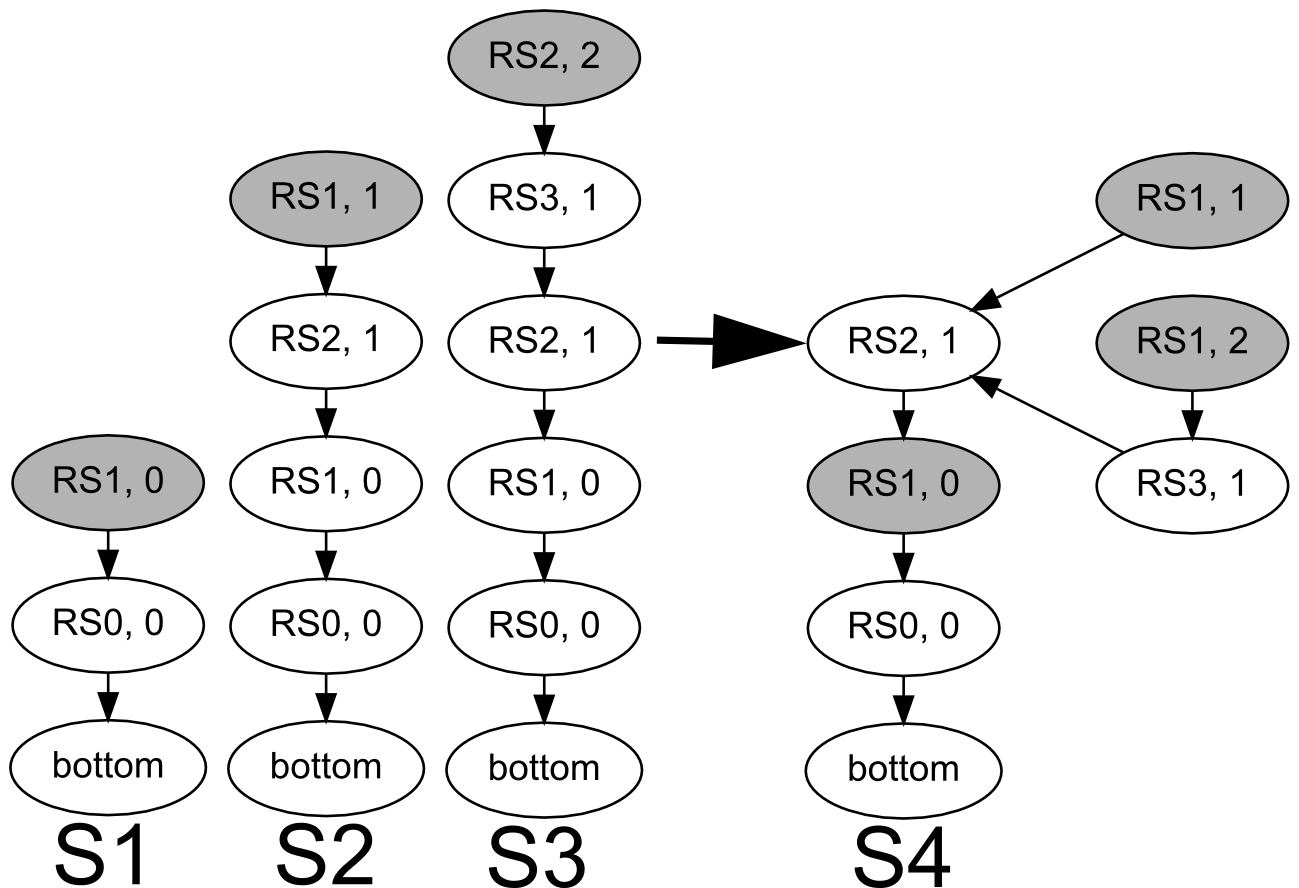
\includegraphics[width=.8\textwidth]{pics/ex_gss.png}
\caption{Пример GSS}
\label{fig:gss} 
\end{center}
\end{figure}

\subsection{Сжатое представление леса разбора}

Для переиспользования общих поддеревьев вывода Ян Рекерс (Jan Rekers, University of Amsterdam) предложил сжатое представление леса разбора (Shared Packed Parse Forest, SPPF)~\cite{SPPF}, которое позволяет компактно представлять множество деревьев вывода. Важным свойством SPPF является то, что из него можно извлечь только те и только те деревья, которые могли быть получены в результате построения вывода конкретного входа в заданной грамматике. Для обеспечения этого свойства в SPPF, кроме терминальных и нетерминальных узлов, добавляются дополнительные узлы различных типов. Конкретный набор типов дополнительные узлов может отличаться в зависимости от алгоритма анализа.

\fvset{frame=lines,framesep=5pt}
\begin{listing}
% * <Екатерина Вербицкая> 17:30:32 02 Jul 2015 UTC+0300:
% Ты вроде вводил правила как нечто со стрелкой, так и выдерживай стиль дальше в тексте.
    \begin{pyglist}[numbers=left,numbersep=5pt]

s ::= m 
s ::= p
p ::= A n
m ::= A l
l ::= n
n ::= B C

\end{pyglist}
\caption{Грамматика $G_1$}
\label{lst:g1}
\end{listing}


Пример SPPF для грамматики $G_1$ (листинг~\ref{lst:g1}) и входа \verb|ABC| приведён на рисунке~\ref{fig:ex_sppf}. Представлены два различных дерева вывода~(\ref{fig:ex_sppf1} и ~\ref{fig:ex_sppf2}) и результат их объединения в SPPF~\ref{fig:ex_sppf3}. Узлы с именами вида ``n <name>'' --- это нетерминальные узлы, ``е <name>'' --- терминальные, ``prod <num>'' --- дополнительные узлы, показывающие, согласно какой продукции из грамматики прозводился вывод нетерминала, являющегося предком данного узла.  

\begin{figure}[h!]
\centering
   \begin{subfigure}[b]{0.3\textwidth}
       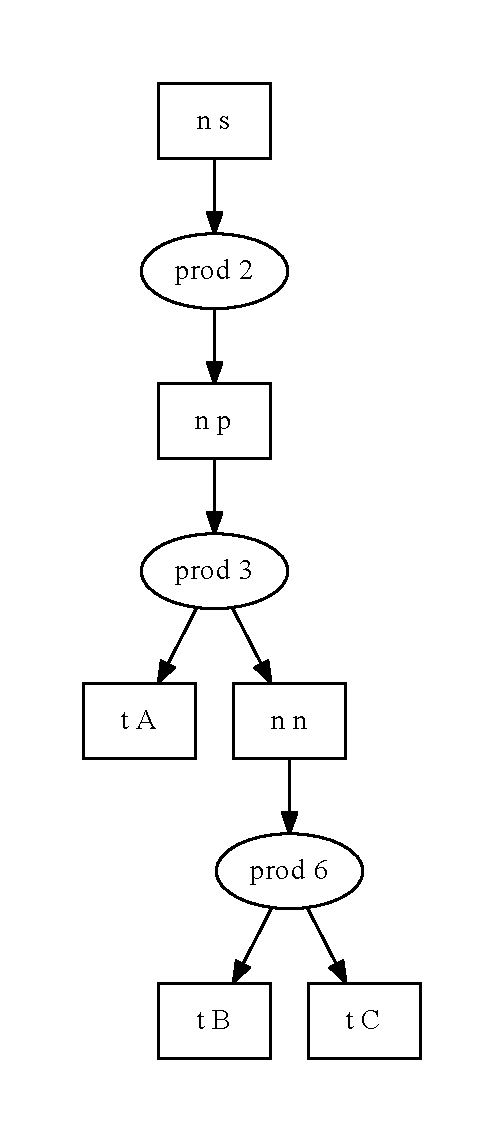
\includegraphics[width=\textwidth]{pics/ex_sppf1}
       \caption{Первое дерево вывода}
       \label{fig:ex_sppf1}
   \end{subfigure}
   ~ 
   \begin{subfigure}[b]{0.3\textwidth}
       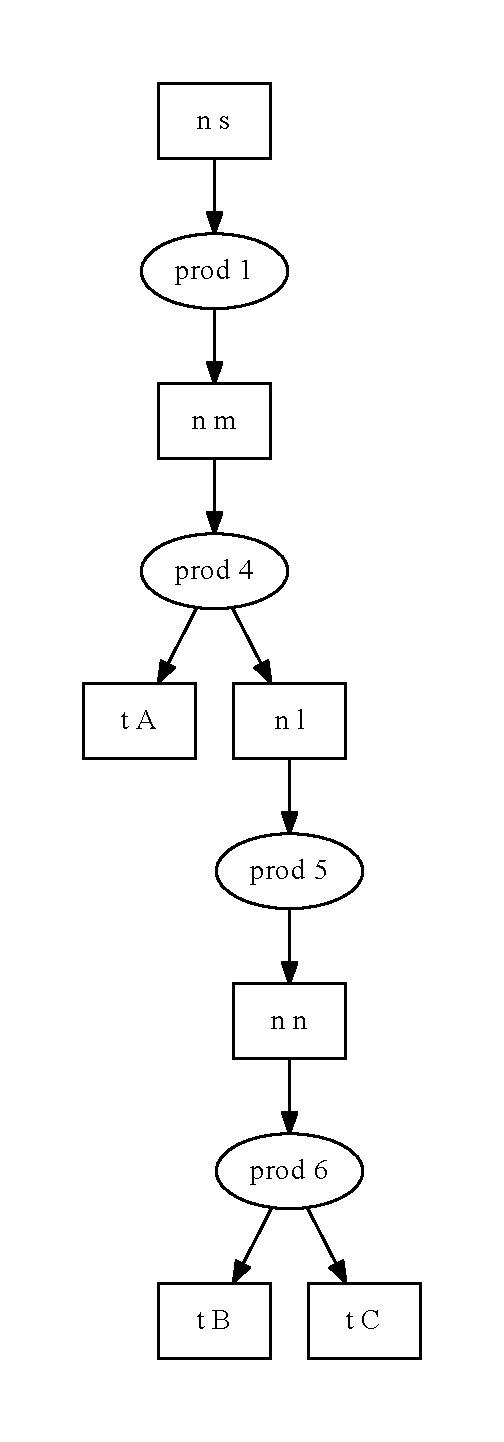
\includegraphics[width=\textwidth]{pics/ex_sppf2}
       \caption{Второе дерево вывода}
       \label{fig:ex_sppf2}
   \end{subfigure}
   ~
   \begin{subfigure}[b]{0.3\textwidth}
       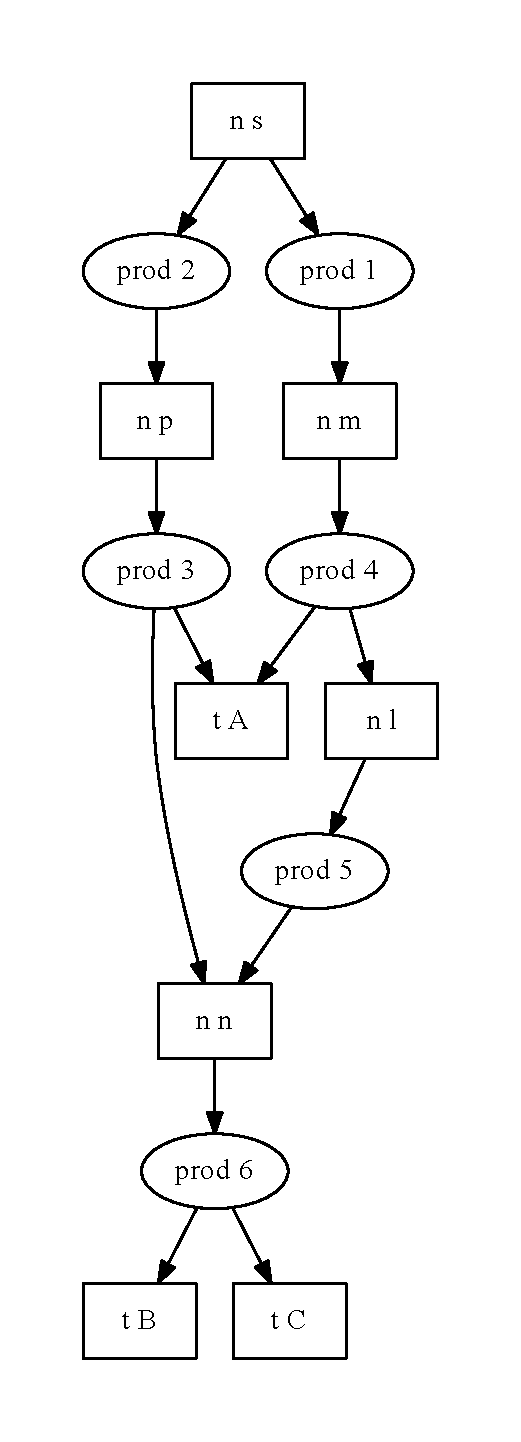
\includegraphics[width=\textwidth]{pics/ex_sppf3}
       \caption{Объединение деревьев вывода в SPPF}
       \label{fig:ex_sppf3}
   \end{subfigure}
   \caption{Пример SPPF для грамматики $G_1$ и входа \textbf{\texttt{ABC}}}
   \label{fig:ex_sppf} 
\end{figure}

\subsection{Алгоритм RNGLR}

RNGLR-алгоритм (Right-Nulled Generalized LR)~\cite{RNGLR} является модификацией предложенного Масару Томитой алгоритма, который не был способен обрабатывать все контекстно-свободные грамматики. Чтобы устранить данный недостаток, Элизабет Скотт (Elizabeth Scott) и Адриан Джонстон (Adrian Johnstone) из университета Royal Holloway (Великобритания) предложили RNGLR-алгоритм, который расширяет GLR-алгоритм специальным способом обработки обнуляемых справа правил (right-nullable rules, имеющих вид $\mathrm{A} \rightarrow \alpha \beta$, где $\beta$ выводит пустую строку $\epsilon$), позволяя обрабатывать произвольные контекстно-свободные грамматики. Алгоритм синтаксического анализа динамически формируемых выражений, представленный в данной работе, основан на RNGLR-алгоритме. Его подробное описание в виде псевдокода приведено ниже.

\begin{listing}[!ht]
\hrule
\begin{algorithmic}[1]
%\caption{RNGLR-алгоритм}
%\label{rnglr}
\Function{parse}{$grammar, input$}
  \State{$\mathcal{R} \gets \emptyset$} \Comment{Очередь троек: вершина GSS, нетерминал, длина свёртки}
  \State{$\mathcal{Q} \gets \emptyset$} \Comment{Коллекция пар: вершина GSS, состояние синтаксического анализатора}
  \If{$input = \epsilon$}
    \If{$grammar$ accepts empty input} {report success}
    \Else { report failure}
    \EndIf
  \Else
    \State{\Call{addVertex}{$0, 0, startState$}}
    \ForAll{$i$ in $0..input.Length-1$}
      \State{\Call{reduce}{$i$}}
      \State{\Call{push}{$i$}}
    \EndFor
    \If{$i=input.Length-1$ and there is a vertex in the last level of GSS which state is accepting}
      \State{report success}
    \Else { report failure}
    \EndIf
  \EndIf
\EndFunction
\Function{reduce}{$i$}
  \While{$\mathcal{R}$ is not empty}
    \State{$(v, N, l) \gets \mathcal{R}.Dequeue()$}
    \State{find the set $\mathcal{X}$ of vertices reachable from $v$ along the path of length $(l-1)$}
    \State{or length $0$ if $l=0$}
    \ForAll{$v_{h} = (level_{h}, state_{h})$ in $\mathcal{X}$}
      \State{$state_{t} \gets$ calculate new state by $state_{h}$ and nonterminal $N$}
      \State{\Call{addEdge}{$i, v_{h}, v.level, state_{tail}, (l=0)$}}
    \EndFor
  \EndWhile
\EndFunction
\Function{push}{$i$}
  \State{$\mathcal{Q^{'}} \gets$ copy $\mathcal{Q}$}
  \While{$\mathcal{Q^{'}}$ is not empty}
    \State{$(v, state) \gets \mathcal{Q}.Dequeue()$}
    \State{\Call{addEdge}{$i, v, v.level + 1, state, false$}}
  \EndWhile
\EndFunction
\end{algorithmic}
\hrule
  \caption{Критерии сравнения инструментов анализа динамически формируемых строковых выражений}\label{lst:metricsForComparison}
\end{listing}

\begin{listing}[!ht]
\hrule

\begin{algorithmic}[1]
\caption{Построение GSS}
\label{RNGLRMain}
\Function{addVertex}{$i, level, state$}
  \If{GSS does not contain vertex $v = (level, state)$}
    \State{add new vertex $v = (level, state)$ to GSS}
    \State{calculate the set of shifts by $v$ and the $input[i+1]$ and add them to $\mathcal{Q}$}
    \State{calculate the set of zero-reductions by $v$ and the $input[i+1]$ and}
    \State{add them to $\mathcal{R}$}
  \EndIf
  \State{\Return{$v$}}
\EndFunction
\Function{addEdge}{$i, v_{h}, level_{t}, state_{t}, isZeroReduction$}
  \State{$v_{t} \gets$ \Call{addVertex}{$i, level_{t}, state_{t}$}}
  \If{GSS does not contain edge from $v_{t}$ to $v_{h}$}
    \State{add new edge from $v_{t}$ to $v_{h}$ to GSS}
    \If{not $isZeroReduction$}
      \State{calculate the set of reductions by $v$ and the $input[i+1]$ and}
      \State{add them to $\mathcal{R}$}
    \EndIf
  \EndIf
\EndFunction
\end{algorithmic}

\hrule
\end{listing}

Для эффективного представления множества стеков во время синтаксического анализа в алгоритме RNGLR, как и в классическом GLR, используется структурированный в виде графа стек (GSS). Вершина GSS~--- это пара $(s,l)$, где $s$~--- состояние синтаксического анализатора, а $l$~--- уровень (позиция во входном потоке).

RNGLR-алгоритм последовательно считывает символы входного потока слева направо, по одному за раз, и строит GSS по ``слоям'': сначала осуществляются все возможные свёртки для данного символа, после чего сдвигается следующий символ со входа. Свёртка или сдвиг модифицируют GSS следующим образом. Предположим, что в GSS необходимо добавить ребро $(v_t,v_h)$. По построению, конечная вершина добавляемой дуги к такому моменту уже обязательно находится в GSS. Если начальная вершина также содержится в GSS, то в граф добавляется новое ребро (если оно ранее не было добавлено), иначе создаются и добавляются в граф и начальная вершина, и ребро. Каждый раз, когда создаётся новая вершина $v=(s,l)$, алгоритм вычисляет новое состояние синтаксического анализатора $s'$ по $s$ и следующему символу входного потока. Пара $(v,s')$, называемая push, добавляется в глобальную коллекцию $\mathcal{Q}$. Также при добавлении новой вершины в GSS вычисляется множество $\epsilon$-свёрток, после чего элементы этого множества добавляются в глобальную очередь $\mathcal{R}$. Свёртки длины $l>0$ вычисляются и добавляются в $\mathcal{R}$ каждый раз, когда создаётся новое (не-$\varepsilon$) ребро. Подробное описание работы со структурированным в виде графа стеком GSS пердставлено в листинге~\ref{RNGLRMain}.

В силу неоднозначности грамматики входная строка может иметь несколько деревьев вывода, как правило, содержащих множество идентичных поддеревьев. Для того, чтобы компактно хранить множество деревьев вывода, используется SPPF, являющееся ориентированным графом и в данном случае обладающее следующей структурой.
\begin{enumerate}
  \item \emph{Корень} соответствует стартовому нетерминалу грамматики.
  \item \emph{Терминальные} вершины, не имеющие исходящих дуг, соответствуют либо терминалам грамматики, либо деревьям вывода пустой строки $\varepsilon$.
  \item \emph{Нетерминальные} вершины являются корнем дерева вывода некоторого нетерминала грамматики; только вершины-продукции могут быть непосредственно достижимы из таких вершин.
  \item \emph{Вершины-продукции}, представляющие правую часть правила грамматики для соответствующего нетерминала. Вершины, непосредственно достижимые из них, упорядочены и могут являться либо терминальными, либо нетерминальными вершинами. Количество таких вершин лежит в промежутке $[l-k \dots l]$, где $l$~--- это длина правой части продукции, а $k$~--- количество финальных символов, выводящих $\varepsilon$. При этом такие символы игнорируются для уменьшения потребления памяти.
\end{enumerate}

SPPF создаётся параллельно с построением GSS. С каждым ребром GSS ассоциирован либо терминальный, либо нетерминальный узел. Когда добавление ребра в GSS происходит во время операции push, новая терминальная вершина создаётся и ассоциируется с ребром. Нетерминальные вершины ассоциируются с рёбрами, добавленными во время операции reduce. Если ребро уже есть в GSS, к ассоциированной с ним нетерминальной вершине добавляется новая вершина-продукция. Подграфы, ассоциированные с рёбрами пути, вдоль которого осуществлялась свёртка, добавляются как дети к вершине-продукции. После того, как входной поток прочитан до конца, производится поиск всех вершин, имеющих принимающее состояние анализатора, после чего подграфы, ассоциированные с исходящими из таких вершин рёбрами, объединяются в один граф. Из полученного графа удаляются все недостижимые из корня вершины, в результате чего остаются только корректные деревья разбора для входной строки. 

Листинг~\ref{rnglr} представляет более детальное описание алгоритма.

    
\section{Используемые инструменты}

В этом разделе описываются основные инструменты, использованные в работе: YaccConstructor~\cite{YCArticle, YCUrl}, выбранный в качастве основы для реализации алгоритма синтаксического анализа динамически формируемых выражений, и ReSharper SDK~\cite{ReSharperSDK}, использованный для разработки сшиений для microsoft Visual Studio IDE.  

\subsection{YaccConstructor}\label{YCDescr}

    Одной из задач данной работы является создание инструментария, упрощающего разработку целевых инструментов статического анализа строковых выражений, которые включают такие этапы, как лексический и синтаксический анализ. При создании лексических и синтаксических анализаторов широко распространённой практикой является использование генераторов, которые по описанию языка строят соответствующий анализатор. Данный подход должен быть реализован и для создания инструментов анализа встроенных языков.
    Работа с описаниями языков программирования --- грамматикой и лексический спецификацией --- в рамках решаемой задачи аналогична работе с ними в стандартных генераторах. По этой причине необходимо было выбрать готовую платформу для работы с грамматиками и создания синтаксических и лексических анализаторов.

        В качестве такой платформы был выбран исследовательский проект лаборатории языковых инструментов JetBrains YaccConstructor (YC)~\cite{YCArticle, YCUrl}, который является модульной платформой с открытым исходным кодом для исследований в области лексического и синтаксического анализа и разработки соответствующих инструментов. YC реализован на платформе Microsoft .NET\footnote{Microsoft .NET --- платформа для разработки программных продуктов компании Microsoft. Общие сведения о платформе: \url{https://msdn.microsoft.com/ru-ru/library/zw4w595w(v=vs.110).aspx} (Посещено 23.06.2015.)}, основной язык разработки --- F\#\footnote{F\# --- функциональный язык программирования для платформы .NET. Информация о языке: \url{http://fsharp.org} (Посещено 23.06.2015.)}~\cite{FSharp}.

\begin{figure}[h!]
\begin{center}
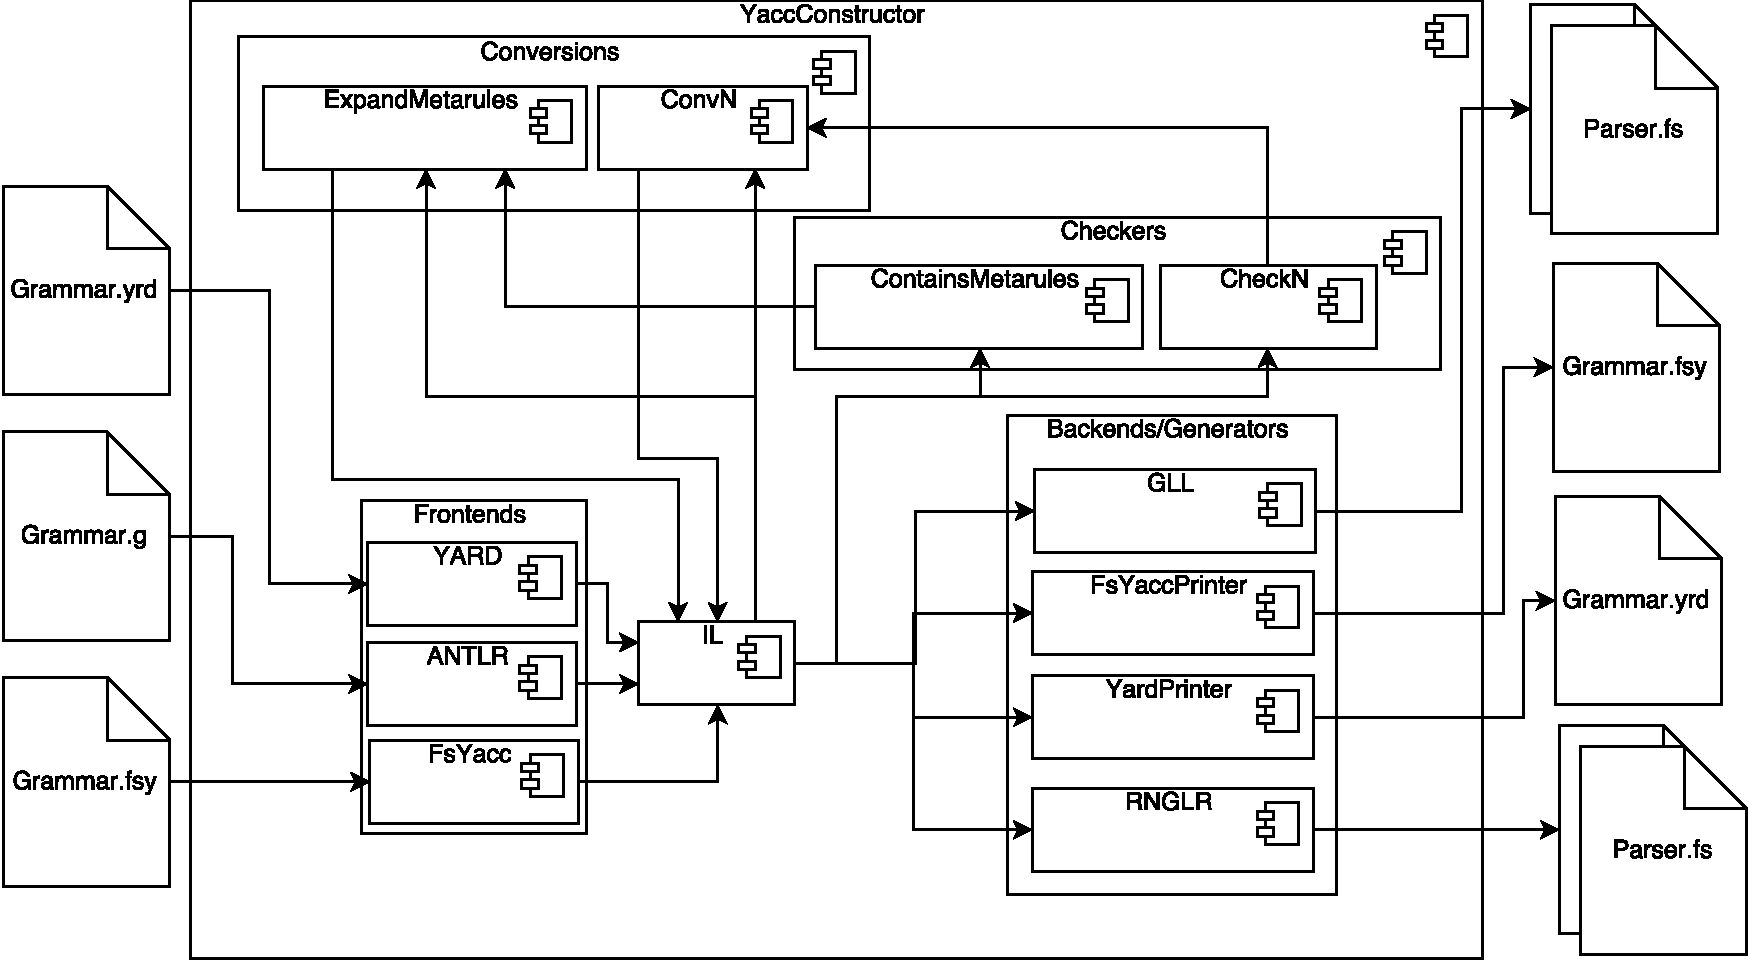
\includegraphics[width=\textwidth]{pics/YCArch.pdf}
\caption{Архитектура платформы YaccConstructor}
\label{fig:ycarch} 
\end{center}
\end{figure}

        
    Архитектура YC, представленная на рисунке~\ref{fig:ycarch}, позволяет собирать требуемый инструмент из существующих модулей: можно выбрать фронтенд, соответствующий используемому языку спецификации грамматики, задать необходимые преобразования грамматики, указать необходимый генератор. Генераторы (backend) представляют различные инструменты, которые по внутреннему представлению грамматики получают результ, полезный для конечного пользователя. Например, это могут быть генераторы синтаксических анализаторов, основанные на различных алгоритмах или принтеры, генерирующие текст грамматики в определённом формате или на заданном языке. YC является расширяемой платформой: модуль любого типа может быть реализован, в том числе с переиспользованием уже существующих, и подключён к платформе.  

    В рамках YC разработан выразительный язык спецификации грамматик YARD, поддерживающий атрибутные грамматики, грамматики в EBNF~\footnote{EBNF --- расфиренная форма Бэкуса-Наура. Грамматики в этой форме позволяют использовать регулярные выражения в правых частях правил~\cite{EBNFISO}.} и многое другое. В листинге~\ref{lst:calcExample} представлена грамматика языка арифметических выражений Calc на языке YARD.  

\fvset{frame=lines,framesep=5pt}
\begin{listing}
    \begin{pyglist}[numbers=left,numbersep=5pt]
    
    [<Start>]
    expr: factor [MULT expr]
    powExpr: NUM | LBR expr RBR
    factor: powExpr [POW factor]
    
\end{pyglist}
\caption{Пример грамматики языка арифметических выражений на языке YARD}
\label{lst:calcExample}
\end{listing}


    Выразительный синтаксис языка описания грамматики удобен для разработчика, однако генераторы, как правило, не поддерживают обработку грамматик в таком виде. Часто требуется, чтобы правая часть правила  грамматики не содержала регулярных выражений, а состояла бы из цепочки из терминалов и нетерминалов. Это необходимо для работы алгоритма построения таблиц. Для решения этой задачи в YC реализован ряд преобразований грамматик. В результате их применения к грамматике, представленной в листинге~\ref{lst:calcExample}, можно получить грамматику, представленную в листинге~\ref{lst:calcTransformExample}.


\fvset{frame=lines,framesep=5pt}
\begin{listing}
    \begin{pyglist}[numbers=left,numbersep=5pt]
    
    [<Start>]
    expr: factor 
    expr: factor MULT expr
    powExpr: NUM 
    powExpr: LBR expr RBR
    factor: powExpr
    factor: powExpr POW factor
    startRule: expr

\end{pyglist}
\caption{Пример преобразованной грамматики языка арифметических выражений}
\label{lst:calcTransformExample}
\end{listing}

    Также в рамках платформы YC в качестве одного из модулей ранее был реализован генератор синтаксических анализаторов на основе RNGLR-алгоритма. Это позволяет переиспользовать общие функции и структуры данных при разработке анализатора для встроенных языков. 
    Таким образом, алгоритм анализа встроенных языков и соответствующий генератор может быть реализован в рамках платформы YC в качестве одного из модулей. При этом можно использовать готовый язык описания грамматики и преобразования, а также переиспользовать необходимые элементы генератора анализаторов на основе RNGLR-алгоритма. Таким образом, YC был выбран в качестве основы для реализации благодаря удобной архитектуре и большому количеству готовых решений. 


\subsection{ReSharper SDK}\label{ReSharperSDKDescr}

    Для демонстрации разработанного в рамках данной работы инструмента представляется целесообразным создать на его основе целевое решение. Для этого необходимо окружение, способное обрабатывать внешний язык, поскольку такие операции над внешним языком, как построение дерева разбора, базовый анализ (например, построение графа потока управления или графа потока данных), лежат за пределами рассматриваемой в данной работе задачи, и их выполнение должно осуществляться сторонними инструментами. При этом такие инструменты должны предоставлять необходимую для решения основной задачи функциональность. Кроме того, необходимо иметь удобный способ взаимодействия с пользователем: необходимо получать код для анализа и отображать результаты в виде, удобном для пользователя. Один из самых распространённых способов работы с программным кодом --- это работа в интегрированной среде разработки.

    Так как реализация работы велась на платформе Microsoft .NET, то соответствующее окружение для обработки внешнего языка и организации взаимодействия с пользователем на данной платформе должно работать на данной платформе. Одной из самых известных сред разработки для платформы .NET, позволяющей создавать расширения на .NET языках, является Microsoft Visual Studio IDE\footnote{Сайт среды разработки Microsoft Visual Studio IDE: \url{https://www.visualstudio.com/} (Посещён 23.06.2015.)}. Она и была выбрана в качестве цели для интеграции инструмента статического анализа строковых выражений. Однако у данной среды разработки достаточно сложный механизм создания расширений, что вызвано его универсальностью. При решении нашей задачи универсальность не требовалась, поэтому можно было бы использовать менее универсальный и более простой механизм.

Такой механизм предоставляется ReSharper SDK~\cite{ReSharperSDK}.  ReSharper~\cite{ReSharper} --- расширение для Microsoft Visual Studio, предоставляющее пользователю широкий набор дополнительных анализов кода. Для разработчиков предоставляется свободно распространяемая SDK, реализующая анализ таких языков, как C\#, VB.NET и др. Большая часть функциональности ReSharper выделена в свободно распространяемую SDK, что даёт возможность сторонним разработчикам создавать собственные расширения к ReSharper, переиспользуя его функциональность. В контексте данной работы это позволяет упростить создание плагинов для поддержки различных встроенных языков. Кроме того, ReSharper SDK предоставляет более удобную ``обёртку'' над многими интерфейсами Microsoft Visual Studio, что упрощает взаимодействие с ней и полезно, например, при предоставлении результатов пользователю.

Следует также отметить, что ReSharper является многоязыковым инструментом, то есть поддерживает большой набор различных языков и спроектирован так, чтобы максимально упростить поддержку новых языков. Это позволяет создавать инструменты, обрабатывающие не только различные встроенные языки, но также и различные внешние.

 Выделим следующую функциональность ReSharper SDK, необходимую для реализации поддержки встроенных языков в Microsoft Visual Studio.  
\begin{itemize}
    \item Построение дерева разбора внешнего языка (C\#, JavaScript и другие, поддерживаемые ReSharper), узлы которого содержат координаты в исходном коде, что позволяет точно связывать текстовое и структурное представление кода.
    \item Анализ потока данных и анализ потока управления для поддерживаемых языков. На основе существующих анализов можно строить более сложные, необходимые, например, для построения регулярной аппроксимации.
    \item Вывод сообщений об ошибках и графическое выделение некорректных мест в текстовом редакторе.
    \item Взаимодействие с редактором кода, позволяющее настраивать подсветку синтаксиса, получать позицию курсора и управлять ею, что нужно для динамической подсветки парных элементов.
\end{itemize}

Таким образом ReSharper SDK и Microsoft Visual Studio IDE выбраны в качестве основы для разработки целевого инструмента на основе представленных в данной работе результатов.

\section{Выводы}

На основе проведённого обзора можно сделать следующие выводы, обосновывающие необходимость проведения исследований в области статического анализа динамически формируемых строковых выражений.

\begin{itemize}
    \item Проблема анализа строковых выражений актуальна в нескольких областях: поддержка встроенных языков в интегрированных средах разработки, оценка качества кода, содержащего динамически формируемые строковые выражения, реинжиниринг программного обеспечения.
    \item Большинство реализаций поддерживают конкретный внешний и конкретный встроенный язык и, как правило, решают одну достаточно узкую задачу. При этом, зачастую, плохо расширяемы, как в смысле поддержки других языков, так и в смысле решения новых задач. Полноценные средства разработки инструментов статического анализа динамически формируемых выражений, упрощающие создание решений для новых языков, отсутствуют.
    \item Для эффективного решения этих задач необходимо структурное представление кода, однако на текущий момент не представлено законченного решения, позволяющего строить деревья вывода для динамически формируемых выражений.
\end{itemize}

Кроме того, обзор позволяет выявить следующие подходы, технологии и средства.

\begin{itemize}
    \item В качестве приближения множества значений целесообразно использовать регулярную аппроксимацию~\cite{JSA, RegOverApprox}, так как при работе с ней ряд важных задач является разрешимым в общем случае, что не верно для контекстно-свободной. Более того, работа с регулярной аппроксимацией упрощает решение такой задачи, как лексический анализ встроенных языков.
    \item Лексический и синтаксический анализы должны быть разделены. Это оправдано как с теоретической, так и с практической точек зрения, так как лексический анализ не привносит потери точности и упрощается переиспользование спецификаций языков и самих анализаторов. 
    \item В качестве основы алгоритма синтаксического анализа днамически формируемых выражений можно выбрать алгоритм обобщённого синтаксического анализа~\cite{GeneralisedlrBIG}, так как в нём реализовано эффективное управление множеством стеков и деревьев разбора, что важно при работе с динамически формируемыми выражениями.
\end{itemize}
\clearpage

\section{Синтаксический анализ контекстно-свободной аппроксимации}

Наш алгоритм принимает на вход управляющие таблицы LL-анализа, построенные по эталонной грамматике, и GFG, который является представлением КС-грамматики --- аппроксимации множества значений выражения. 
Мы переиспользуем основные структуры данных и функции описанного ранее алгоритма анализа регулярной аппроксимации на основе GLL, расширяя данный подход для корректной обработки GFG.

Алгоритм последовательно обходит узлы GFG, производя синтаксический анализ порождаемых им строк. 
Для правильного построения таких строк, согласно определению выводимости строки в GFG-грамматике, для каждого просматриваемого пути необходимо поддерживать баланс call- и return-узлов. 
То есть, при прохождении пути алгоритм должен манипулировать дополнительным стеком (назовем его \textit{CR-стеком}). 
При достижении call-узла в стек добавляется номер return-узла, соответствующего ему; при достижении end-узла необходимо снять со стека номер return-узла и продолжить обход из него. 

Для экономии памяти мы не храним CR-стек для каждой из текущих ветвей работы алгоритма (напомним, что GLL-алгоритм может одновременно рассматривать несколько вариантов разбора строки). 
Вместо этого множество CR-стеков, по аналогии с основным стеком GLL-анализатора, представляется в виде GSS. 
Пример можно увидеть на рисунке \ref{fig:gss}. GSS позволяет хранить только одну копию общих префиксов нескольких стеков, каждый путь в нем соответствует отдельному CR-стеку.

\begin{figure}[h]
	\centering
	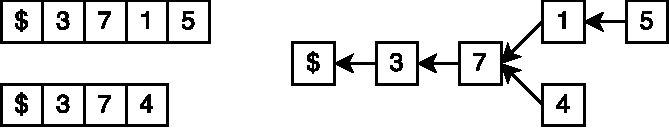
\includegraphics[width=6cm]{pictures/gss_cr}
	\caption{Структурированный в виде графа стек}
	\label{fig:gss}
\end{figure}

Для хранения указателя на текущую вершину стека мы добавили в дескрипторы дополнительное поле. 
Таким образом, дескриптором в нашем алгоритме называется пятерка вида $(L, u, i, N, s)$, где $i$ --- номер вершины GFG, $s$ --- указатель на вершину CR-стека в GSS, остальные поля аналогичны тем, которые представлены в дескрипторах оригинального GLL-алгоритма.

Другой особенностью работы с GFG является то, что он, в отличие от регулярной аппроксимации --- детерминированного конечного автомата, допускает возможность неоднозначного выбора пути обхода. 
Подобная ситуация возникает при наличии в исходной грамматике нескольких продукций, содержащих в левой части одинаковый нетерминал. 
Например, GFG на рисунке \ref{fig:gfg} содержит start-узел под номером 3, из которого выходит два ребра с пустой меткой (аналог $\epsilon$-переходов в конечном автомате).

Механизм дескрипторов позволяет решать проблему недетерминированного выбора пути --- для каждого из возможных вариантов создается отдельный дескриптор, который добавляется в очередь исполнения. 
Вернемся к примеру с узлом 3 на рисунке \ref{fig:gfg}. Пусть в текущий момент времени мы имеем дескриптор $(L_1, u_1, i_1, N_1, s_1)$. 
При рассмотрении ребер, выходящих из узла 3, будут созданы дескрипторы $(L_1, u_1, 4, N_1, s_1)$ и $(L_1, u_1, 5, N_1, s_1)$. Если ранее такие дескрипторы не создавались (для контроля за этим в GLL поддерживается глобальное множество создаваемых дескрипторов), они будут добавлены в очередь.

Функции \textbf{dispatcher} и \textbf{add} (проверка и добавление в очередь дескриптора) алгоритма анализа регулярной аппроксимации были незначительно изменены нами для работы с расширенными дескрипторами. 
Функция \textbf{processing} и методы для работы с основным стеком и построения SPPF переиспользованы без изменений.
Обработка start/call/exit-узлов и контроль за состоянием CR-стеков были реализованы во вспомогательной функции \textbf{closure}, псевдокод которой приведен ниже.
Она исполняется перед вызовами \textbf{dispatcher} и \textbf{processing}, производя рекурсивный обход GFG до тех пор, пока не встретит start- или scan-узел. 
При достижении start-узла создаются дескрипторы для каждого из возможных путей, и управление переходит к \textbf{dispatcher};
scan-узел обрабатывается функцией \textbf{processing} так же, как и вершина конечного автомата в оригинальном алгоритме.

\section{Closure properties of languages with polynomial rational indices}
\label{sec:closure}
Given a context-free language $L$ with a polynomial rational index, it is interesting to find which language operations preserve this property.  Boasson et al. \cite{RatBasic} give following useful relations for polynomial indices of two languages $L$ and $L'$.
\begin{theorem}[\cite{RatBasic}]
Context-free languages with polynomial rational indices are closed under intersection with a regular language, union, concatenation, homomorphism and inverse homomorphism. More precisely,
\begin{itemize}
\item $\rho_{L \cup L'} \le  \max{(\rho_L, \rho_{L'})} $
\item $\rho_{LL'} \le \rho_L + \rho_{L'}$
\item $\rho_{L \cap R}(n) \le \rho_L(nm)$, where $R$ is a regular language recognised by an $m$-state automaton
\item $\rho_{h(L)}(n) \le \rho_L(n)$ and $\rho_{h^{-1}(L)}(n) < n(\rho_L(n) +1)$, where $h: \Sigma^* \rightarrow \Delta^*$ is a homomorphism.
\end{itemize}
\end{theorem}
From the relations above it is easy to see that the family of context-free languages with polynomial rational indices is a full trio. Every full trio is closed under prefix and quotient with regular languages. Obviously, CFLs with polynomial rational indices languages are closed under reversal.  Next we show that context-free languages with polynomial rational indices are closed under Kleene star and insertion of a regular language (or context-free language with a polynomial rational index).
\begin{theorem}
Context-free languages with polynomial rational indices are closed under Kleene star and insertion of a regular language  (or context-free language with a polynomial rational index). Particularly,
\begin{itemize}
\item $\rho_{L^*}(n) \le n(\rho_L(n))$
\item $\rho_{LL'} \le \rho_L + \rho_{L'}$
\end{itemize}
\end{theorem}
\begin{proof}
\textit{Kleene star.} Let $G = (\Sigma, N, P, S)$ and $L(G)$ be a language with polynomial rational index. Consider language $L^{+}$, which grammar $G_1$ has the start nonterminal $S_1$. By definition of the Kleene plus operation, a rightmost derivation from $S_1$ generates a sequence of one or more start nonterminals $S$ from $G$, each of which generates some string in $L(G)$. Let $D$ be a directed labelled graph with $n$ nodes. Suppose there are nodes $u$ and $v$ in $D$ such that:
\begin{enumerate}
\item $v$ is not $L(G)$-reachable from $u$ and
\item $v$ is  $L^+$-reachable from $u$
\end{enumerate}
Then $v$ is reachable from $u$ via concatenation of words in $L(G)$. Consider the longest shortest path $u\pi_1 v$ between $u$ and $v$. It can be obtained by joining $(S, u, i), (S, i, j), ..., (S, w, v)$ into $(S_1, u, v)$.  If $L$ has the polynomial rational index, then for every realizable triple $(A, i, j)$ corresponding shortest path $i \pi j$ has at most polynomial length. There are no more than $O(n)$ such triples in concatenation because there are no repetitions of the same node in the sequence of start and end nodes of triples (otherwise $u\pi_1 v$ is not the shortest path, for example, path $u \rightarrow i \rightarrow k \rightarrow l \rightarrow i \rightarrow j \rightarrow v$ can be replaced with shorter path $u \rightarrow i  \rightarrow j \rightarrow v$), so $u\pi_1 v$ has at most polynomial length. In other words, we have $\rho_{L^+}(n) \le n(\rho_L(n))$.
\\
Family of languages with polynomial rational indices is a full trio closed under union, concatenation and Kleene star, therefore it is a full ALF. Full AFLs is known to be closed under substitution.
\\
\textit{Insertion of a regular language.} To prove closure under insertion of a regular language, the following PDA can be constructed. Let $L$ be a context-free language with polynomial rational index and let $M$ be a PDA recognizing $L$. New PDA $M'$ for insertion of a regular language $R$ recognized by finite automation $F$ into $L$ can be obtained as follows: duplicate all states in $M$, initial state is placed in first set and final states reside in the second set. Every state in the first set has its own copy of outgoing arcs of the initial state of $F$. Every ingoing arc of final state of $F$ is connected directly to every state of the second set of $M$. In other words, every state from the first set is the initial state of $F$ and every state from the second set is a final state of $F$. All arcs from $F$ are labelled the same way as they are labelled in $F$.
Consider intersection of $M'$ and arbitrary finite automotion $F'$ with $n$ states. The longest non-empty shortest path $i \pi j$ in the intersection of $M'$ and $F'$ consists of three sub-paths: $i\pi_1k$, $k\pi_2m$ and $m\pi_3j$, where $i\pi_1k$ ($m\pi_3j$) is the shortest paths in the intersection of $F'$ and first (second) set of states of $M$ respectively, and $k\pi_2m$ is the shortest path in the intersection of $F'$ and $F$. $k\pi_2m$ has at most polynomial length because all regular languges have polynomial rational indices, $i\pi_1k$ and $m\pi_3j$ have polynomial length because $M$ is a PDA for language with rational index, therefore  $i \pi j$ has polynomial length.
\end{proof}


Using closure properties, it is easier to find new subclasses of context-free languages for which CFL-reachability problem is in NC.
\begin{example}[Metalinear languages \cite{metalinear}.]
\\
Let $G = (\Sigma, N, P, S)$ be a context-free grammar. $G$ is \textit{metalinear} if all productions of $P$ are of the following forms:
\begin{enumerate}
\item $S \rightarrow A_1A_2...A_k$, where $A_i \in N - \{S\}$
\item $A \rightarrow u$, where $A \in N \setminus \{S\}$ and $u \in (\Sigma^*((N \setminus \{S\}) \cup {\varepsilon})\Sigma^*)$
\end{enumerate}


The width of a metalinear grammar is $max\{k$ | $S \rightarrow A_1A_2...A_k \}$. Metalinear languages of width 1 are obviously linear languages. It is easy to see that every metalinear language is a union of concatenations of $k$ linear languages. Linear languages have polynomial rational index,  CFLs with polynomial rational index are closed under concatenation and union, so metalinear languages have polynomial rational index.
\end{example}



Результатом работы алгоритма является SPPF, представляющий набор деревьев разбора строк, порождаемых GFG и одновременно с этим выводимых в эталонной грамматике.
Отметим, что SPPF может быть построен не всегда, так как класс КС-языков не замкнут относительно пересечения.
\section{Conclusion and future work}
In this paper, we shown how the context-free path query evaluation w.r.t. the relational and the single-path query semantics can be reduced to the calculation of matrix transitive closure. Also, we provided a formal proof of the correctness of the proposed reduction. In addition, we introduced an algorithm for computing this transitive closure, which allows us to efficiently apply GPGPU computing techniques. Finally, we shown the practical applicability of the proposed algorithm by running different implementations of our algorithm on real-world data.

We can identify several open problems for further research. In this paper we have considered only two semantics of context-free path querying but there are other important semantics, such as all-path query semantics~\cite{hellingsPathQuerying} which requires to present all paths for all triples $(A,m,n)$. Context-free path querying implemented with algorithm~\cite{GLL} can answer the queries in all-path query semantics by constructing a parse forest. It is possible to construct a parse forest for a linear input by matrix multiplication~\cite{okhotin_cyk}. Whether it is possible to generalize this approach for a graph input is an open question.

In our algorithm, we calculate the matrix transitive closure naively, but there are algorithms for the transitive closure calculation, which are asymptotically more efficient. Therefore, the question is whether it is possible to apply these algorithms for the matrix transitive closure calculation to the problem of context-free path querying.

Also, there are Boolean grammars~\cite{okhotinBoolean}, which have more expressive power than context-free grammars. Boolean path querying is an undecidable problem~\cite{hellingsRelational} but our algorithm can be trivially generalized to work on boolean grammars because parsing with boolean grammars can be expressed by matrix multiplication~\cite{okhotin_cyk}. It is not clear what a result of our algorithm applied to Boolean grammars would look like. Our hypothesis is that it would produce the upper approximation of a solution.

From a practical point of view, matrix multiplication in the main loop of the proposed algorithm may be performed on different GPGPU independently. It can help to utilize the power of multi-GPU systems and increase the performance of context-free path querying.

There is an algorithm~\cite{apspGPU} for transitive closure calculation on directed graphs which generalized to handle graph sizes inherently larger then the DRAM memory available on the GPU. Therefore, the question is whether it is possible to apply this approach to the matrix transitive closure calculation in the problem of context-free path querying.

\bibliographystyle{abbrv}
\bibliography{biblio}

\section{Dataset description}\label{section:dataset}

In our evaluation we use dataset which contains the following parts.
{\setlength{\tabcolsep}{0.4em}
	\begin{table}[h]
		\caption{RDFs properties}
		\label{tbl:propRDF}
		\rowcolors{2}{}{lightgray}
		\begin{tabular}{| l | c | c | c | c |}
			\hline
			Name                  & \#V    & \#E     & \#type &\#subClassOf \\
			\hline
			\hline
			atom-primitive				& 291		& 685		& 138	& 122	\\
			univ-bench					& 179		& 413		& 84		& 36		\\
			travel						& 131		& 397		& 90		& 30		\\
			skos							& 144		& 323		& 70		& 1		\\
			people\_pets					& 337		& 834		& 161	& 33		\\
			generations					& 129		& 351		& 78		& 0		\\
			foaf							& 256		& 815		& 174	& 10		\\
			biomed-mesure-prim   	    & 341		& 711		& 130	& 122	\\
			funding						& 778		& 1480		& 304	& 90               \\
			pizza						& 671		& 2604		& 365	& 259              \\
			wine							& 733		& 2450		& 485	& 126              \\
			core							& 1323		& 8684		& 1412	& 178              \\
			pathways						& 6238		& 37196		& 3118 	& 3117             \\
			go-hierarchy					& 45007		& 1960436	& 0		& 490109           \\
			enzyme						& 48815		& 219390		& 14989	& 8163             \\
			eclass\_514en				& 239111		& 1047454	& 72517	& 90962            \\
			go							& 272770		& 1068622	& 58483	& 90512            \\
			\hline
		\end{tabular}
	\end{table}
}

{\setlength{\tabcolsep}{0.4em}
\begin{table*}[h]
\caption{RDFs query $G_2$ (time is measured in seconds and memory is measured in megabytes)}
\label{tbl:tableRDFQ2}
\rowcolors{3}{}{lightgray}
\begin{tabular}{| l | r  r | r  r | r  r | r  r | r  r |}
    \hline

    \multirow{3}{*}{Name}   &   \multicolumn{6}{|c|}{Relational semantics index}	&	\multicolumn{4}{|c|}{Single path semantics index} \\
    \cline{2-11}
    &	\multicolumn{2}{|c|}{RG\_CPU\textsubscript{rel}}	&	\multicolumn{2}{|c|}{RG\_CUSP\textsubscript{rel}}	&	\multicolumn{2}{|c|}{RG\_SPARSE\textsubscript{rel}} &	\multicolumn{2}{|c|}{RG\_CPU\textsubscript{path}}	&	\multicolumn{2}{|c|}{RG\_SPARSE\textsubscript{path}}	 \\
    \cline{2-11}
    &   Time & Mem &  Time     & Mem & Time     & Mem  &  Time     & Mem & Time     & Mem \\
    \hline
    \hline
    atom-primitive          & 0.001 & 0.3  & 0.001 & 0.1 & 0.002 & 0.1   & 0.001 & 0.3  & 0.002 & 0.1   \\
biomedical-mesure-primitive & 0.002 & 0.1  & 0.014 & 2.0   & 0.009 & 0.1   & 0.006 & 0.1  & 0.012 & 0.1   \\
core                        & 0.001 & 0.3  & 0.006 & 0.1 & 0.004 & 0.1   & 0.003 & 0.3  & 0.005 & 0.1   \\
eclass\_514en               & 0.035 & 6.5  & 0.020 & 16.0  & 0.100   & 12.0    & 0.123 & 17.7 & 0.127 & 18.0    \\
enzyme                      & 0.006 & 3.9  & 0.006 & 0.6 & 0.010  & 0.1   & 0.012 & 5.3  & 0.008 & 0.4   \\
foaf                        & 0.001 & 0.1  & 0.004 & 0.1 & 0.002 & 0.1   & 0.001 & 0.1  & 0.003 & 0.1   \\
funding                     & 0.002 & 0.1  & 0.015 & 0.4 & 0.007 & 0.1   & 0.009 & 0.1  & 0.008 & 0.1   \\
generations                 & 0.001 & 0.1  & 0.001 & 0.1 & 0.001 & 0.1   & 0.001 & 0.1  & 0.001 & 0.1   \\
go-hierarchy                & 0.095 & 17.8 & 0.253 & 528.0 & 0.175 & 130.4 & 0.884 & 88.8 & 0.306 & 138.8 \\
go                          & 0.306 & 25.8 & 0.240 & 84.0  & 0.181 & 25.4  & 0.918 & 78.1 & 0.219 & 34.2  \\
pathways                    & 0.005 & 0.2  & 0.005 & 0.4 & 0.004 & 0.1   & 0.017 & 0.5  & 0.003 & 0.1   \\
people\_pets                & 0.001 & 0.1  & 0.007 & 0.1 & 0.004 & 0.1   & 0.001 & 0.1  & 0.005 & 0.1   \\
pizza                       & 0.002 & 0.3  & 0.012 & 0.2 & 0.008 & 0.1   & 0.010  & 0.3  & 0.009 & 0.1   \\
skos                        & 0.001 & 0.1  & 0.001 & 0.1 & 0.001 & 0.1   & 0.001 & 0.1  & 0.002 & 0.1   \\
travel                      & 0.001 & 0.1  & 0.007 & 0.1 & 0.005 & 0.1   & 0.001 & 0.1  & 0.005 & 0.1   \\
univ-bench                  & 0.001 & 0.1  & 0.007 & 0.1 & 0.005 & 0.1   & 0.001 & 0.1  & 0.005 & 0.1   \\
wine                        & 0.001 & 0.3  & 0.006 & 0.1 & 0.004 & 0.1   & 0.002 & 0.3  & 0.004 & 0.1  \\
    \hline
  \end{tabular}
\end{table*}
}

\begin{itemize}
\item The real-world data RDFs provided in CFPQ\_Data dataset\footnote{CFPQ\_Data dataset GitHub repository: \url{https://github.com/JetBrains-Research/CFPQ_Data}. Access date: 12.11.2019.} from~\cite{Mishin:2019:ECP:3327964.3328503}.
\item Geospecies (RDF which contains information about biological hierrarchy\footnote{The Geospecies RDF: \url{https://old.datahub.io/dataset/geospecies}. Access date: 12.11.2019.} and same-generation query over \textit{broaderTransitive} relation) is provided in~\cite{Kuijpers:2019:ESC:3335783.3335791} and integrated in our evaluation with CFPQ\_Data.
\item It was shown in~\cite{Mishin:2019:ECP:3327964.3328503} that matrix-based algorithm is performant enough to handle bigger RDFs than those used in the initial datasets, such as~\cite{RDF}.
So, we add several big RDFs to CFPQ\_Data and use them in our evaluation.
New RDFs: \textit{go-hierarchy, go, enzime, core, pathways} are from UniProt database\footnote{Protein sequences data base: \url{https://www.uniprot.org/}. RDFs with data are avalable here: \url{ftp://ftp.uniprot.org/pub/databases/uniprot/current_release/rdf}. Access date: 12.11.2019}, and \textit{eclass-514en} is from eClassOWL project\footnote{eClassOWL project: \url{http://www.heppnetz.de/projects/eclassowl/}. eclass-514en file is available here: \url{http://www.ebusiness-unibw.org/ontologies/eclass/5.1.4/eclass_514en.owl}. Access date: 12.11.2019.}.
\end{itemize}

The properties of the RDFs from the dataset are given in table \ref{tbl:propRDF}. 
Geospecies RDF contains 450609 vertices, 2311461 edges, and 20867 edges labeled by \textit{broaderTransitive}.
Note that while the number of edges labeled by \textit{broaderTransitive} is equal to provided in~\cite{Kuijpers:2019:ESC:3335783.3335791}, the total number of vertices and edges is bigger. It is because we naively convert each triple from RDF to edge in the graph, while J. Kuijpers et al. use special \textit{neosemantics}\footnote{Neosemantix is an RDF processing plugin for Neo4j. Web page: \url{https://neo4j.com/labs/nsmtx-rdf/}. Access date: 30.03.2020.} plugin which can, for example, handling multivalued properties accurately.  

The variants of the \textit{same-generation query}~\cite{FndDB} are used in almost all cases because it is an important example of real-world queries that are context-free but not regular.
So, variations of the same generation query are used in our evaluation.
All queries are added to the CFPQ\_Data dataset.

We use two queries over \textit{subClassOf} and \textit{type} relations.
The first query is the grammar $G_1$:
\[
 \begin{array}{lcl}
   s  \rightarrow \textit{subClassOf}^{\ -1} \ s \ \textit{subClassOf}   & \quad & s  \rightarrow \textit{type}^{\ -1} \ s \ \textit{type}     \\
   s  \rightarrow \textit{subClassOf}^{\ -1} \ \textit{subClassOf}       & \quad & s  \rightarrow  \textit{type}^{\ -1}  \ \textit{type}

 \end{array}
 \]
The second one is the grammar $G_2$: \[s \rightarrow \textit{subClassOf}^{\ -1} \ s \ \textit{subClassOf} \mid \textit{subClassOf}\]

For geospecies we use same-generation query \textit{geo} from the original paper~\cite{Kuijpers:2019:ESC:3335783.3335791}: \[s \rightarrow \textit{broaderTransitive} \ s \ \textit{broaderTransitive}^{\ -1} \]
\[s \rightarrow \textit{broaderTransitive}  \ \textit{broaderTransitive}^{\ -1} \]


\section{Evaluation Details}

Results for RDFs querying with $G_2$ grammar are presented in table~\ref{tbl:tableRDFQ2}.
We can see, that for small graphs time for both relational and single-path querying are similar for CPU and GPGPU versions, but for bigger graphs (\textit{go} and \textit{go-hierarchy}, for example) GPUPU version is more performant than CPU one.

\balance



\end{document}